\section{张量网络基础}\label{chapter:basics}

随着阶数升高，张量的表示与运算都变得更加复杂。
张量网络（tensor network, TN）为处理这类高阶对象提供了高效的框架，使表示与分析同时得到简化。
张量网络的图示记法（graphical notation）让复杂张量运算的可视化与化简变得直观~\citep{orus2014practical,biamonte2017tensor}。
本节用张量网络的语言介绍张量的基本概念与常见的张量运算。

\subsection{什么是张量网络？}
顾名思义，张量网络就是把张量彼此连接而成的网络。更准确地说，张量网络是一类图：顶点表示\emph{张量}，边表示\emph{已收缩}的指标（contracted indices），即共享的模。张量网络的图示记法最早由~\cite{penrose1971applications}提出。张量用带腿（leg，也称边 edge）的图形表示，例如，
$
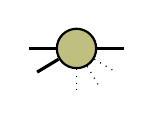
\begin{tikzpicture}[baseline=-0.5ex]
    \tikzset{tensor/.style = {minimum size = 0.5cm,shape = circle,thick,draw=black,inner sep = 0pt}, edge/.style = {thick,line width=.4mm},every loop/.style={}}
    \def\x{6}
    \node[tensor,fill=green!50!red!50!white] (T) at (\x,0) {$\Tt$};
    \draw[edge] (T) -- (\x-0.6,0);
    \draw[edge] (T) -- (\x+0.6,0);
    \draw[edge] (T) -- (\x-0.5,-0.3);
    \draw[dotted] (T) -- (\x,-0.6);
    \draw[dotted] (T) -- (\x+0.5,-0.3);
    \draw[dotted] (T) -- (\x+0.3,-0.5);
    \end{tikzpicture}.
$
我们用矩形、三角形、圆形等不同形状以及各种颜色来表示张量。形状与颜色主要起视觉提示的作用。
张量的\emph{阶}（order）指它的维度个数。例如，$N$ 阶张量 $\Tt\in\RR^{d_1\times\cdots\times d_N}$ 是由标量~$\Tt_{i_1,\dots,i_N}$ 构成的多维数组，由 $N$ 个指标 $i_1\in [d_1], i_2\in[d_2],\cdots, i_N \in [d_N]$ 索引。每个轴称为张量的一个\emph{模}（mode）：$N$ 阶张量有 $N$ 个模。
 
 张量把向量与矩阵自然推广为高维数组。阶数越高，这类数组的表示就越困难。\emph{张量网络}为表示和运算这些高阶对象提供了简单而直观的方式。借助张量网络的图示记法，可以更轻松地表达复杂的张量运算~\citep{biamonte2017tensor,orus2014practical}。


\paragraph{张量网络的节点}\label{def:tn-nodes}
在张量网络中，每个节点（node，或称顶点）表示一个张量，腿~（与之关联的边）的数目对应张量的阶：标量是没有边的节点，向量节点有一条边，矩阵节点有两条边，依此类推。例如，
\begin{center}
    
    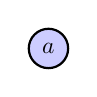
\begin{tikzpicture}[baseline=-0.5ex]
    \tikzset{tensor/.style = {minimum size = 0.5cm,shape = circle,thick,draw=black,inner sep = 0pt}, edge/.style = {thick,line width=.4mm},every loop/.style={}}
    \def\y{0}
    \def\x{0}
    \node[tensor,fill=blue!20!white] (a) at (\x,\y){\scalebox{0.85}{$a$}};
    \end{tikzpicture}%
    \ \ \ $\in \RR$,\hspace{0.01cm}
    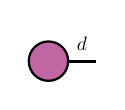
\begin{tikzpicture}[baseline=-0.5ex]
    \tikzset{tensor/.style = {minimum size = 0.5cm,shape = circle,thick,draw=black,inner sep = 0pt}, edge/.style = {thick,line width=.4mm},every loop/.style={}}
    \def\y{0}
    \def\x{0}
    \node[tensor,fill=blue!40!red!60!white] (a) at (\x,\y){\scalebox{0.85}{$\ab$}};
    \draw[edge] (\x+0.25,\y) -- (\x+0.6,\y)  node [midway,above] {\scalebox{0.7}{\dimcolor{$d$}}};
    \end{tikzpicture}
    $\in \RR^d$,\hspace{0.3cm}
    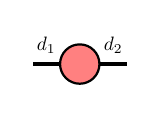
\begin{tikzpicture}[baseline=-0.5ex]
    \tikzset{tensor/.style = {minimum size = 0.5cm,shape = circle,thick,draw=black,inner sep = 0pt}, edge/.style = {thick,line width=.4mm},every loop/.style={}}
    \def\y{0}
    \def\x{0}
    \node[tensor,fill=red!50!white] (A) at (\x,\y){\scalebox{0.85}{$\Ab$}};
    \draw[edge] (\x+0.25,\y) -- (\x+0.6,\y)  node [midway,above] {\scalebox{0.7}{\dimcolor{$d_2$}}};
    \draw[edge] (\x-0.25,\y) -- (\x-0.6,\y)  node [midway,above] {\scalebox{0.7}{\dimcolor{$d_1$}}};
    \end{tikzpicture}
    \ \ \ $\in \RR^{d_1\times d_2}$,\hspace{0.3cm}
    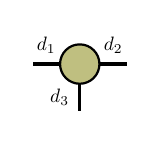
\begin{tikzpicture}[baseline=-0.5ex]
    \tikzset{tensor/.style = {minimum size = 0.5cm,shape = circle,thick,draw=black,inner sep = 0pt}, edge/.style = {thick,line width=.4mm},every loop/.style={}}
    \def\y{0}
    \def\x{0}
    \node[tensor,fill=green!50!red!50!white] (A) at (\x,\y){\scalebox{0.85}{$\At$}};
    \draw[edge] (\x+0.25,\y) -- (\x+0.6,\y)  node [midway,above] {\scalebox{0.7}{\dimcolor{$d_2$}}};
    \draw[edge] (\x-0.25,\y) -- (\x-0.6,\y)  node [midway,above] {\scalebox{0.7}{\dimcolor{$d_1$}}};
    \draw[edge] (\x,\y-0.25) -- (\x,\y-0.6)  node [midway,left] {\scalebox{0.7}{\dimcolor{$d_3$}}};
    \end{tikzpicture}
    \ \ \ $\in \RR^{d_1\times d_2\times d_3}$,\hspace{0.01cm}
    \begin{tikzpicture}[baseline=-0.5ex]
    \tikzset{tensor/.style = {minimum width = 1.8cm,minimum height = 0.4cm,shape = rounded rectangle,thick,draw=black,inner sep = 0pt}, edge/.style = {thick,line width=.4mm},every loop/.style={}}
    \def\x{0}
    \def\y{0}
    \draw[edge] (\x-0.2,\y-0.15) -- (\x-0.2,\y-0.6)node [midway,left=-0.05cm] {\scalebox{0.7}{\dimcolor{$d_2$}}};
    \draw[edge] (\x-0.6,\y-0.15) -- (\x-0.6,\y-0.6)node [midway,left=-0.05cm] {\scalebox{0.7}{\dimcolor{$d_1$}}};
    \draw[edge] (\x+0.2,\y-0.15) -- (\x+0.2,\y-0.6)node [midway,left=-0.05cm] {\scalebox{0.7}{\dimcolor{$d_3$}}};
    \draw[edge] (\x+0.6,\y-0.15) -- (\x+0.6,\y-0.6)node [midway,left=-0.05cm] {\scalebox{0.7}{\dimcolor{$d_4$}}};
    \node[tensor,fill=green!30!white] (Bt) at (\x,\y){$\Bt$};
    \end{tikzpicture}
    $\in \RR^{d_1\times d_2\times d_3\times d_4}$.

\end{center}
分别表示标量、向量、矩阵、三阶张量与四阶张量。
在本手册中，
\begin{itemize}
    \item 张量用带颜色的图形表示，称为节点，颜色与形状并无特定含义~（除非另有说明）。
    \item 标量用小写字母表示~（如 $a$），向量用粗小写字母表示~（如 $\vb$），矩阵用粗大写字母表示（如 $\Mb$），高阶张量则用
    粗花体大写字母表示~（如 $\Tt$）。
    \item 张量每个模的维数用一个灰色字母标在相应腿的上方，例如，
$
    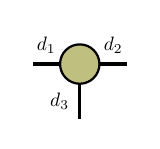
\begin{tikzpicture}[baseline=-0.5ex]
    \tikzset{tensor/.style = {minimum size = 0.5cm,shape = circle,thick,draw=black,inner sep = 0pt}, edge/.style = {thick,line width=.4mm},every loop/.style={}}
    \def\y{0}
    \def\x{0}
    \node[tensor,fill=green!50!red!50!white] (A) at (\x,\y){\scalebox{0.85}{$\At$}};
    \draw[edge] (\x+0.25,\y) -- (\x+0.6,\y)  node [midway,above] {\scalebox{0.7}{\dimcolor{$d_2$}}};
    \draw[edge] (\x-0.25,\y) -- (\x-0.6,\y)  node [midway,above] {\scalebox{0.7}{\dimcolor{$d_1$}}};
    \draw[edge] (\x,\y-0.25) -- (\x,\y-0.7)  node [midway,left] {\scalebox{0.7}{\dimcolor{$d_3$}}};
    \end{tikzpicture}
    \ \ \ \in \RR^{d_1\times d_2\times d_3},
$
是尺寸为 $d_1\times d_2\times d_3$ 的三阶张量。
    
$
\At_{i,j,k} = 
    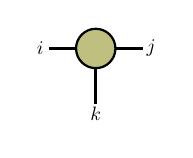
\begin{tikzpicture}[baseline=-0.5ex]
    \tikzset{tensor/.style = {minimum size = 0.5cm,shape = circle,thick,draw=black,inner sep = 0pt}, edge/.style = {thick,line width=.4mm},every loop/.style={}}
    \def\y{0}
    \def\x{0}
    \node[tensor,fill=green!50!red!50!white] (A) at (\x,\y){\scalebox{0.85}{$\At$}};
    \draw[edge] (\x+0.25,\y) -- (\x+0.6,\y)  node [pos=1.3] {\scalebox{0.7}{\indcolor{$j$}}};
    \draw[edge] (\x-0.25,\y) -- (\x-0.6,\y)  node [pos=1.3] {\scalebox{0.7}{\indcolor{$i$}}};
    \draw[edge] (\x,\y-0.25) -- (\x,\y-0.7)  node [pos=1.3] {\scalebox{0.7}{\indcolor{$k$}}};
    \end{tikzpicture}
$    
是三阶张量 $\At$ 的第 $(i,j,k)$ 个元素。
\end{itemize}
注意，大矩阵有时也可借助重排（reshaping）被视为高阶张量，例如，
\begin{align*}
    &\Tb
    =
    \begin{tikzpicture}[baseline=\baseline]
    \tikzset{tensor/.style = {minimum size = 0.5cm,shape = circle,thick,draw=black,inner sep = 0pt}, edge/.style = {thick,line width=.4mm},every loop/.style={}}
    \def\x{0}
    \def\y{0}
    \node[tensor,fill=green!50!blue!40!white] (Tb) at (\x,\y){$\Tb$};
    \draw[edge] (Tb) -- (\x+1.15,\y) node [midway,above] {\scalebox{0.7}{\dimcolor{$J_1J_2J_3J_4$}}};
    \draw[edge] (Tb) -- (\x-1.15,\y) node [midway,above] {\scalebox{0.7}{\dimcolor{$I_1I_2I_3I_4$}}};
    \end{tikzpicture}\in\RR^{I_1I_2I_3I_4\times J_1J_2J_3J_4}
    \equiv
    \Tt = 
    \begin{tikzpicture}[baseline=-0.5ex]
    \tikzset{tensor/.style = {minimum width = 1.8cm,minimum height = 0.4cm,shape = rounded rectangle,thick,draw=black,inner sep = 0pt}, edge/.style = {thick,line width=.4mm},every loop/.style={}}
    \def\x{0}
    \def\y{0}
    \draw[edge] (\x-0.2,\y-0.15) -- (\x-0.2,\y-0.6)node [midway,left=-0.05cm] {\scalebox{0.7}{\dimcolor{$I_2$}}};
    \draw[edge] (\x-0.6,\y-0.15) -- (\x-0.6,\y-0.6)node [midway,left=-0.05cm] {\scalebox{0.7}{\dimcolor{$I_1$}}};
    \draw[edge] (\x+0.2,\y-0.15) -- (\x+0.2,\y-0.6)node [midway,left=-0.05cm] {\scalebox{0.7}{\dimcolor{$I_3$}}};
    \draw[edge] (\x+0.6,\y-0.15) -- (\x+0.6,\y-0.6)node [midway,left=-0.05cm] {\scalebox{0.7}{\dimcolor{$I_4$}}};
    \draw[edge] (\x-0.2,\y+0.15) -- (\x-0.2,\y+0.6)node [midway,left=-0.05cm] {\scalebox{0.7}{\dimcolor{$J_2$}}};
    \draw[edge] (\x-0.6,\y+0.15) -- (\x-0.6,\y+0.6)node [midway,left=-0.05cm] {\scalebox{0.7}{\dimcolor{$J_1$}}};
    \draw[edge] (\x+0.2,\y+0.15) -- (\x+0.2,\y+0.6)node [midway,left=-0.05cm] {\scalebox{0.7}{\dimcolor{$J_3$}}};
    \draw[edge] (\x+0.6,\y+0.15) -- (\x+0.6,\y+0.6)node [midway,left=-0.05cm] {\scalebox{0.7}{\dimcolor{$J_4$}}};
    \node[tensor,fill=yellow] (Bt) at (\x,\y){$\Tt$};
    \end{tikzpicture}
    \in\RR^{I_1\times I_2\times I_3\times I_4\times J_1 \times J_2\times J_3\times J_4}.
\end{align*}
\paragraph{张量网络的边}\label{subsec:contraction} 在张量网络图中，腿分为两类：已收缩的腿~（连接两个张量的腿）与未收缩的腿，后者也称自由腿~（free legs），一端悬空~（即不与任何其他张量相连的腿）。如前所述，未收缩的腿对应自由指标（free index）：自由腿的数目给出张量的阶——标量没有自由腿，向量有一条，矩阵有两条，高阶张量则有三条或更多。已收缩的腿表示收缩（contraction）：
张量可沿尺寸相同的腿相连，这表示对所连接的模求和~（收缩）。
求和与收缩在本文中通用。最常见的收缩运算为\textit{矩阵乘法}。对两个矩阵 $\Ab\in\RR^{d_1\times R}, \Bb\in\RR^{R\times d_2}$，其矩阵乘积相当于 $\Ab$ 的第二模与 $\Bb$ 的第一模之间的收缩：

\begin{align}\label{eq:matrix-product}
(\Ab\Bb)_{ij} 
=
\begin{tikzpicture}[baseline=\baseline]
   \tikzset{tensor/.style = {minimum size = 0.5cm,shape = circle,thick,draw=black,inner sep = 0pt}, edge/.style = {thick,line width=.4mm},every loop/.style={}}
    \def\y{0}
    \def\x{0}
    \node[tensor,fill=red!50!white] (A) at (\x,\y){\scalebox{0.85}{$\Ab$}};
    \node[tensor,fill=blue!50!white] (B) at (\x+1,\y){\scalebox{0.85}{$\Bb$}};
    \draw[edge] (A) -- (B) node [above,midway] {\scalebox{0.7}{\dimcolor{$R$}}};
    \draw[edge] (\x-0.25,\y) -- (\x-0.75,\y)  node [pos=1.3] {\scalebox{0.7} {\indcolor{$i$}}};
    \draw[edge] (\x+1.25,\y) -- (\x+1.75,\y)  node [pos=1.3] {\scalebox{0.7}{\indcolor{$j$}}};
    \end{tikzpicture}
= \sum_{r=1}^R\Ab_{ir}\Bb_{rj},\ \ \ \text{for}\ \ i\in[d_1],j\in[d_2]\ .
\end{align}
由于该等式对一切指标 $i$ 与 $j$ 都成立，可以直接简写为
\begin{align}\label{eq:matrix-product_noidx}
\Ab\Bb 
=
\begin{tikzpicture}[baseline=\baseline]
   \tikzset{tensor/.style = {minimum size = 0.5cm,shape = circle,thick,draw=black,inner sep = 0pt}, edge/.style = {thick,line width=.4mm},every loop/.style={}}
    \def\y{0}
    \def\x{0}
    \node[tensor,fill=red!50!white] (A) at (\x,\y){\scalebox{0.85}{$\Ab$}};
    \node[tensor,fill=blue!50!white] (B) at (\x+1,\y){\scalebox{0.85}{$\Bb$}};
    \draw[edge] (A) -- (B) node [above,midway] {\scalebox{0.7}{\dimcolor{$R$}}};
    \draw[edge] (\x-0.25,\y) -- (\x-0.75,\y)  node [midway, above] {\scalebox{0.7}{\dimcolor{$d_1$}}};
    \draw[edge] (\x+1.25,\y) -- (\x+1.75,\y)  node [midway,above] {\scalebox{0.7}{\dimcolor{$d_2$}}};
    \end{tikzpicture}
 \ \in \mathbb R^{d_1\times d_2}.
\end{align}

 在上图中可以看到，尺寸同为 $R$ 的两条腿相互连接。这与矩阵乘法相一致：矩阵乘法就是对维度相同的指标求和。最后，由于所得的图有两条自由腿，它表示一个矩阵。这里的最终对象是一个矩阵，而矩阵可以用单个节点表示，这说明在张量网络中节点可以被合并：
$$
\Ab\Bb =\Mb \Leftrightarrow 
\begin{tikzpicture}[baseline=\baseline]
   \tikzset{tensor/.style = {minimum size = 0.5cm,shape = circle,thick,draw=black,inner sep = 0pt}, edge/.style = {thick,line width=.4mm},every loop/.style={}}
    \def\y{0}
    \def\x{0}
    \node[tensor,fill=red!50!white] (A) at (\x,\y){\scalebox{0.85}{$\Ab$}};
    \node[tensor,fill=blue!50!white] (B) at (\x+1,\y){\scalebox{0.85}{$\Bb$}};
    \draw[edge] (A) -- (B) node [above,midway] {\scalebox{0.7}{\dimcolor{$R$}}};
    \draw[edge] (\x-0.25,\y) -- (\x-0.75,\y)  node [midway, above] {\scalebox{0.7}{\dimcolor{$d_1$}}};
    \draw[edge] (\x+1.25,\y) -- (\x+1.75,\y)  node [midway,above] {\scalebox{0.7}{\dimcolor{$d_2$}}};
    \node[draw=none] () at (\x+2,\y) {\scalebox{1}{\textcolor{black}{$=$}}};
    \node[tensor,fill=blue!30!red!20!white] (M) at (\x+3,\y){\scalebox{0.85}{$\Mb$}};
    \draw[edge] (M) -- (\x+3.75,\y)  node [midway,above] {\scalebox{0.7}{\dimcolor{$d_2$}}};
    \draw[edge] (M) -- (\x+2.25,\y)  node [midway,above] {\scalebox{0.7}{\dimcolor{$d_1$}}};
    \end{tikzpicture}.
$$
矩阵之间的收缩可以直接推广到矩阵与向量、张量与矩阵、张量与矩阵及向量的收缩等情形。下面给出若干张量网络例子及其对应的数学表达式：
\begin{align}\label{eq:matvec}
\Ab\in\RR^{d_1\times R},\vb\in\RR^{R} \ : \ \
\begin{tikzpicture}[baseline=\baseline]
   \tikzset{tensor/.style = {minimum size = 0.5cm,shape = circle,thick,draw=black,inner sep = 0pt}, edge/.style = {thick,line width=.4mm},every loop/.style={}}
    \def\y{0}
    \def\x{0}
    \node[tensor,fill=red!50!white] (A) at (\x,\y){\scalebox{0.85}{$\Ab$}};
    \node[tensor,fill=blue!10!white] (v) at (\x+1,\y){\scalebox{0.85}{$\vb$}};
    \draw[edge] (A) -- (v) node [above,midway] {\scalebox{0.7}{\dimcolor{$R$}}};
    \draw[edge] (\x-0.25,\y) -- (\x-0.75,\y)  node [pos=1.3]{\scalebox{0.7}{\indcolor{$i$}}};
    \end{tikzpicture}
=\sum_{r=1}^R\Ab_{ir}\vb_r,
\end{align}
\begin{align}\label{eq:tenmat}
\At\in\RR^{d_1\times R\times d_2},\Ab\in\RR^{R\times d_3}\ :\ \
\begin{tikzpicture}[baseline = \baseline]
    \tikzset{tensor/.style = {minimum size = 0.5cm,shape = circle,thick,draw=black,inner sep = 0pt}, edge/.style = {thick,line width=.4mm},every loop/.style={}}
    \def\y{0}
    \def\x{0}
    \node[tensor,fill=green!50!red!50!white] (At) at (\x,\y){\scalebox{0.85}{$\At$}};
    \node[tensor,fill=red!50!white] (A) at (\x+1,\y){\scalebox{0.85}{$\Ab$}};
    \draw[edge] (At) -- (A) node [above,midway] {\scalebox{0.7}{\dimcolor{$R$}}};
    \draw[edge] (\x-0.25,\y) -- (\x-0.75,\y)  node [pos=1.3] {\scalebox{0.7}{\indcolor{$i$}}};
    \draw[edge] (\x,\y-0.25) -- (\x,\y-0.75)  node [pos=1.3] {\scalebox{0.7}{\indcolor{$j$}}};
    \draw[edge] (\x+1.25,\y) -- (\x+1.75,\y)  node [pos=1.3] {\scalebox{0.7}{\indcolor{$k$}}};
\end{tikzpicture} 
= \sum_{r=1}^R\At_{ijr}\Ab_{rk},
\end{align}
\begin{align}\label{eq:tenmatvec}
\At\in\RR^{d_1\times R\times d_2},\Ab\in\RR^{R\times d_3}, \vb\in\RR^{d_3}&:
   \begin{tikzpicture}[baseline = \baseline]
    \tikzset{tensor/.style = {minimum size = 0.5cm,shape = circle,thick,draw=black,inner sep = 0pt}, edge/.style = {thick,line width=.4mm},every loop/.style={}}
    \def\y{0}
    \def\x{0}
    \node[tensor,fill=green!50!red!50!white] (At) at (\x,\y){\scalebox{0.85}{$\At$}};
    \node[tensor,fill=red!50!white] (A) at (\x+1,\y){\scalebox{0.85}{$\Ab$}};
    \node[tensor,fill=blue!40!red!60!white] (a) at (\x+2,\y){\scalebox{0.85}{$\vb$}};
    \draw[edge] (At) -- (A) node [above,midway] {\scalebox{0.7}{\dimcolor{$R$}}};
    \draw[edge] (A) -- (a) node [above,midway] {\scalebox{0.7}{\dimcolor{$d_3$}}};
    \draw[edge] (\x-0.25,\y) -- (\x-0.75,\y)  node [pos=1.3] {\scalebox{0.7}{\indcolor{$i$}}};
    \draw[edge] (\x,\y-0.25) -- (\x,\y-0.75)  node [pos=1.3] {\scalebox{0.7}{\indcolor{$j$}}};
    \end{tikzpicture} 
= \sum_{r=1}^R\sum_{k=1}^{d_3}\At_{ijr}\Ab_{rk}\ab_{k}.
\end{align}
由上述各图可见，两个节点之间的边表示求和，同时也表明两个张量在相应的模上共享尺寸相同的维度。
如前所述，张量网络中自由腿的数目对应其所表示张量的阶。对前面的例子，我们有

$$
\begin{tikzpicture}[baseline=\baseline]
   \tikzset{tensor/.style = {minimum size = 0.5cm,shape = circle,thick,draw=black,inner sep = 0pt}, edge/.style = {thick,line width=.4mm},every loop/.style={}}
    \def\y{0}
    \def\x{0}
    \node[tensor,fill=red!50!white] (A) at (\x,\y){\scalebox{0.85}{$\Ab$}};
    \node[tensor,fill=blue!10!white] (v) at (\x+1,\y){\scalebox{0.85}{$\vb$}};
    \draw[edge] (A) -- (v) node [above,midway] {\scalebox{0.7}{\dimcolor{$R$}}};
    \draw[edge] (\x-0.25,\y) -- (\x-0.75,\y)  node [midway, above] {\scalebox{0.7}{\dimcolor{$d_1$}}};
    \end{tikzpicture} 
   \in \mathbb R^{d_1},\ \ 
\begin{tikzpicture}[baseline = \baseline]
    \tikzset{tensor/.style = {minimum size = 0.5cm,shape = circle,thick,draw=black,inner sep = 0pt}, edge/.style = {thick,line width=.4mm},every loop/.style={}}
    \def\y{0}
    \def\x{0}
    \node[tensor,fill=green!50!red!50!white] (At) at (\x,\y){\scalebox{0.85}{$\At$}};
    \node[tensor,fill=red!50!white] (A) at (\x+1,\y){\scalebox{0.85}{$\Ab$}};
    \draw[edge] (At) -- (A) node [above,midway] {\scalebox{0.7}{\dimcolor{$R$}}};
    \draw[edge] (\x-0.25,\y) -- (\x-0.75,\y)  node [midway,above] {\scalebox{0.7}{\dimcolor{$d_1$}}};
    \draw[edge] (\x,\y-0.25) -- (\x,\y-0.75)  node [midway,left] {\scalebox{0.7}{\dimcolor{$d_2$}}};
    \draw[edge] (\x+1.25,\y) -- (\x+1.75,\y)  node [midway,above] {\scalebox{0.7}{\dimcolor{$d_3$}}};
\end{tikzpicture} 
\in \mathbb R^{d_1\times d_2 \times d_3},\ \ \text{and}\ \ 
    \begin{tikzpicture}[baseline = \baseline]
    \tikzset{tensor/.style = {minimum size = 0.5cm,shape = circle,thick,draw=black,inner sep = 0pt}, edge/.style = {thick,line width=.4mm},every loop/.style={}}
    \def\y{0}
    \def\x{0}
    \node[tensor,fill=green!50!red!50!white] (At) at (\x,\y){\scalebox{0.85}{$\At$}};
    \node[tensor,fill=red!50!white] (A) at (\x+1,\y){\scalebox{0.85}{$\Ab$}};
    \node[tensor,fill=blue!40!red!60!white] (a) at (\x+2,\y){\scalebox{0.85}{$\vb$}};
    \draw[edge] (At) -- (A) node [above,midway] {\scalebox{0.7}{\dimcolor{$R$}}};
    \draw[edge] (A) -- (a) node [above,midway] {\scalebox{0.7}{\dimcolor{$d_3$}}};
    \draw[edge] (\x-0.25,\y) -- (\x-0.75,\y)  node [midway,above] {\scalebox{0.7}{\dimcolor{$d_1$}}};
    \draw[edge] (\x,\y-0.25) -- (\x,\y-0.75)  node [midway,left] {\scalebox{0.7}{\dimcolor{$d_2$}}};
    \end{tikzpicture} 
\in \mathbb R^{d_1\times d_2}.
$$
 
\paragraph{从数学表达式到张量网络，再回到数学表达式} 张量网络用起来很简单，因为表示腿和节点并没有严格的规则。
在张量网络图中，节点与边可以在平面内任意摆放，重要的只是图的结构。
例如，把矩阵乘法翻译成张量网络图时，关键是保证相连腿的维度一致。例如对 $\Ab\in\RR^{d_1\times R}, \Bb\in\RR^{R\times d_2}$，下面各图表示的都是\emph{同一个}矩阵乘法：
\begin{align*} 
\Ab\Bb
=
\begin{tikzpicture}[baseline=\baseline]
   \tikzset{tensor/.style = {minimum size = 0.5cm,shape = circle,thick,draw=black,inner sep = 0pt}, edge/.style = {thick,line width=.4mm},every loop/.style={}}
    \def\y{0}
    \def\x{0}
    \node[tensor,fill=red!50!white] (A) at (\x,\y){\scalebox{0.85}{$\Ab$}};
    \node[tensor,fill=blue!50!white] (B) at (\x+1,\y){\scalebox{0.85}{$\Bb$}};
    \draw[edge] (A) -- (B) node [midway,above] {\scalebox{0.7}{\dimcolor{$R$}}};;
    \draw[edge] (\x-0.25,\y) -- (\x-0.75,\y) node [midway,above] {\scalebox{0.7}{\dimcolor{$d_1$}}};;
    \draw[edge] (\x+1.25,\y) -- (\x+1.75,\y) node [midway,above] {\scalebox{0.7}{\dimcolor{$d_2$}}};;
    \node[draw=none] () at (\x+1.95,\y) {$=$};
    \node[tensor,fill=red!50!white] (A1) at (\x+2.85,\y){\scalebox{0.85}{$\Ab$}};
    \node[tensor,fill=blue!50!white] (B1) at (\x+3.85,\y){\scalebox{0.85}{$\Bb$}};
    \draw[edge] (A1) -- (B1) node [midway,above] {\scalebox{0.7}{\dimcolor{$R$}}};;
    \draw[edge] (A1) to [out=60,in=60, distance=0.5cm] (\x+2.2,\y);
    \draw[edge] (B1) to [out=60,in=60, distance=0.5cm] (\x+4.4,\y-0.5);
    \node[draw=none] () at (\x+2.4,\y+0.65) {\scalebox{0.7}{\dimcolor{$d_1$}}};
    \node[draw=none] () at (\x+4,\y+0.65) {\scalebox{0.7}{\dimcolor{$d_2$}}};
    \node[draw=none] () at (\x+4.7,\y) {$=$};
    \node[tensor,fill=blue!50!white] (A2) at (\x+5.3,\y){\scalebox{0.85}{$\Bb$}};
    \node[tensor,fill=red!50!white] (B2) at (\x+6.3,\y){\scalebox{0.85}{$\Ab$}};
    \draw[edge] (A2) -- (B2) node [midway,above] {\scalebox{0.7}{\dimcolor{$R$}}};;
    \draw[edge] (A2) -- (\x+5.3,\y+0.75) node [midway,left] {\scalebox{0.7}{\dimcolor{$d_2$}}};
     \draw[edge] (B2) -- (\x+6.3,\y-0.75) node [midway,right] {\scalebox{0.7}{\dimcolor{$d_1$}}};   
     \node[draw=none] () at (\x+7.1,\y) {$=$};
    \node[tensor,fill=red!50!white] (A3) at (\x+7.6,\y+0.5){\scalebox{0.85}{$\Ab$}};
    \node[tensor,fill=blue!50!white] (B3) at (\x+7.6,\y-0.5){\scalebox{0.85}{$\Bb$}};
    \draw[edge] (A3) -- (B3) node [midway,right] {\scalebox{0.7}{\dimcolor{$R$}}};
    \draw[edge] (A3) -- (\x+7.6,\y+1.25) node [midway,left] {\scalebox{0.7}{\dimcolor{$d_1$}}};
    \draw[edge] (B3) -- (\x+7.6,\y-1.25) node [midway,left] {\scalebox{0.7}{\dimcolor{$d_2$}}};
    \end{tikzpicture}.
\end{align*}
注意，由于 $\Ab\in\RR^{d_1\times R}$ 与 $\Bb\in\RR^{R\times d_2}$ 的尺寸限制，二者之间只有一种收缩方式；因此，即使省去边上标注的维数，上面的图也不会有歧义。 

反之，把张量网络图翻译成数学表达式也可能得到多种解释。例如下面这个矩阵乘法图
$
\begin{tikzpicture}[baseline=\baseline]
   \tikzset{tensor/.style = {minimum size = 0.5cm,shape = circle,thick,draw=black,inner sep = 0pt}, edge/.style = {thick,line width=.4mm},every loop/.style={}}
    \def\y{0}
    \def\x{0}
    \node[tensor,fill=red!50!white] (A) at (\x,\y){\scalebox{0.85}{$\Ab$}};
    \node[tensor,fill=blue!50!white] (B) at (\x+1,\y){\scalebox{0.85}{$\Bb$}};
    \draw[edge] (A) -- (B) node [midway,above] {\scalebox{0.7}{\dimcolor{$R$}}};
    \draw[edge] (\x-0.25,\y) -- (\x-0.75,\y) node [midway,above] {\scalebox{0.7}{\dimcolor{$d_1$}}};
    \draw[edge] (\x+1.25,\y) -- (\x+1.75,\y) node [midway,above] {\scalebox{0.7}{\dimcolor{$d_2$}}};
\end{tikzpicture}
$
依据我们为 $\Ab$、$\Bb$ 与结果矩阵选定的形状不同，它有不同的解读：
\begin{itemize}
    \item 若 $\Ab\in\RR^{d_1\times R}, \Bb\in\RR^{R\times d_2}$ 且结果的大小为 $d_1 \times d_2$，则该图表示乘积 $\Ab\Bb$，
    \item 若 $\Ab\in\RR^{R\times d_1}, \Bb\in\RR^{R\times d_2}$ 且结果的大小为 $d_1 \times d_2$，则该图表示乘积 $\Ab^\ts\Bb$，
    \item 若 $\Ab\in\RR^{R\times d_1}, \Bb\in\RR^{R\times d_2}$ 且结果的大小为 $d_2 \times d_1$，则该图表示乘积 $\Bb^\ts\Ab$，
    \item ...
\end{itemize}
因此，把张量网络图翻译成数学表达式时要多加留心。但这也正是张量网络如此有用之处！当我们操作图示而非数学表达式时，就不必在意例如转置这样的问题。

\paragraph{收缩同一节点的两条腿。 } 如前所述，任意两条维度相同的腿都可以连接起来，构成张量网络中的一条边，即使它们属于同一个节点。举例来说，考虑五阶张量 $\Tt\in\mathbb R^{d_1\times d_2 \times d_3 \times d_2 \times d_4}$。它的第 2 个与第 4 个模维度相同，因此可以把二者收缩在一起。所得的张量网络有三条悬空腿，因而表示一个三阶张量： 
\begin{align*}
&\begin{tikzpicture}[baseline=-0.5ex]
    \tikzset{tensor/.style = {minimum width = 1.8cm,minimum height = 0.4cm,shape = rounded rectangle,thick,draw=black,inner sep = 0pt}, edge/.style = {thick,line width=.4mm},every loop/.style={}}
    \def\x{0}
    \def\y{0}
    \draw[edge] (\x-0.4,\y-0.15) -- (\x-0.4,\y-0.5)node [near end,left=-0.05cm] {\scalebox{0.7}{\dimcolor{$d_2$}}};
    \draw[edge] (\x-0.8,\y-0.15) -- (\x-0.8,\y-0.5)node [near end,left=-0.05cm] {\scalebox{0.7}{\dimcolor{$d_1$}}};
    \draw[edge] (\x,\y-0.15) -- (\x,\y-0.5)node [near end,left=-0.05cm] {\scalebox{0.7}{\dimcolor{$d_3$}}};
    \draw[edge] (\x+0.4,\y-0.15) -- (\x+0.4,\y-0.5)node [near end,left=-0.05cm] {\scalebox{0.7}{\dimcolor{$d_2$}}};
    \draw[edge] (\x+0.8,\y-0.15) -- (\x+0.8,\y-0.5)node [near end,left=-0.05cm] {\scalebox{0.7}{\dimcolor{$d_4$}}};
    \node[tensor,fill=green!30!white] (Bt) at (\x,\y){$\Tt$};
    \end{tikzpicture}\in \mathbb R^{d_1\times d_2\times d_3 \times d_2 \times d_4},\ \ \ \ 
  \begin{tikzpicture}[baseline=-0.5ex]
    \tikzset{tensor/.style = {minimum width = 1.8cm,minimum height = 0.4cm,shape = rounded rectangle,thick,draw=black,inner sep = 0pt}, edge/.style = {thick,line width=.4mm},every loop/.style={}}
    \def\x{0}
    \def\y{0}
    \draw[edge] (\x-0.4,\y-0.15) -- (\x-0.4,\y-0.5);
    \draw[edge] (\x-0.8,\y-0.15) -- (\x-0.8,\y-0.5)node [pos=1.3] {\scalebox{0.7}{\indcolor{$i_1$}}};
    \draw[edge] (\x,\y-0.15) -- (\x,\y-0.5)node [pos=1.3] {\scalebox{0.7}{\indcolor{$i_3$}}};
    \draw[edge] (\x+0.4,\y-0.15) -- (\x+0.4,\y-0.5);
    \draw[edge] (\x-0.4,\y-0.5) to [out=270,in=270] (\x+0.4,\y-0.5) node [midway,below=0.7cm] {\scalebox{0.7}{\dimcolor{$d_2$}}};
    \draw[edge] (\x+0.8,\y-0.15) -- (\x+0.8,\y-0.5)node[pos=1.3] {\scalebox{0.7}{\indcolor{$i_4$}}};
    \node[tensor,fill=green!30!white] (Bt) at (\x,\y){$\Tt$};
    \end{tikzpicture} = \sum_{i_2=1}^{d_2} \Tt_{i_1,i_2,i_3,i_2,i_4},   %
    \text{ and }\ \ \
    \begin{tikzpicture}[baseline=-0.5ex]
    \tikzset{tensor/.style = {minimum width = 1.8cm,minimum height = 0.4cm,shape = rounded rectangle,thick,draw=black,inner sep = 0pt}, edge/.style = {thick,line width=.4mm},every loop/.style={}}
    \def\x{0}
    \def\y{0}
    \draw[edge] (\x-0.4,\y-0.15) -- (\x-0.4,\y-0.5);
    \draw[edge] (\x-0.8,\y-0.15) -- (\x-0.8,\y-0.5)node [midway,left=-0.05cm] {\scalebox{0.7}{\dimcolor{$d_1$}}};
    \draw[edge] (\x,\y-0.15) -- (\x,\y-0.5)node [midway,left=-0.05cm] {\scalebox{0.7}{\dimcolor{$d_3$}}};
    \draw[edge] (\x+0.4,\y-0.15) -- (\x+0.4,\y-0.5);
    \draw[edge] (\x-0.4,\y-0.5) to [out=270,in=270] (\x+0.4,\y-0.5) node [midway,below=0.7cm] {\scalebox{0.7}{\dimcolor{$d_2$}}};
    \draw[edge] (\x+0.8,\y-0.15) -- (\x+0.8,\y-0.5)node [midway,left=-0.05cm] {\scalebox{0.7}{\dimcolor{$d_4$}}};
    \node[tensor,fill=green!30!white] (Bt) at (\x,\y){$\Tt$};
    \end{tikzpicture} \in \mathbb R^{d_1\times d_3 \times d_4}.
\end{align*}
收缩一个 $N$ 阶张量的两条腿后，所得张量的阶数为 $N-2$。这与后文将要介绍的\emph{偏迹}（partial trace）概念密切相关。
\subsection{内积、外积、迹与范数}\label{sec:inner-products}
本节借助张量网络说明，内积（inner product）、外积（outer product）、迹（trace）与范数（norm）这些经典概念如何推广到高阶张量。

\paragraph{内积} 与向量之间经典的内积~（欧几里得内积）类似，两个 $N$ 阶张量 $\St,\Tt\in\RR^{d_1\times\dots\times d_N}$ 的内积是它们对应元素乘积之和：
$$ \langle \St,\Tt \rangle = \sum_{i_1=1}^{d_1}\dots\sum_{i_N=1}^{d_N}\St_{i_1\dots i_N}\Tt_{i_1\dots i_N}.$$ 在张量网络图中，对所有维度求和就是把两个张量的所有腿都连接起来。这样得到的张量网络没有自由腿，表示一个标量。例如，对向量 $\ab\in\RR^{d\times 1}, \bb\in\RR^{d\times 1}$ 有
\begin{align}\label{eq:inner-product}
\langle\ab,\bb\rangle = \sum_{i=1}^d\ab_i\bb_i
=
    \begin{tikzpicture}[baseline=\baseline]
   \tikzset{tensor/.style = {minimum size = 0.5cm,shape = circle,thick,draw=black,inner sep = 0pt}, edge/.style = {thick,line width=.4mm},every loop/.style={}}
    \def\y{0}
    \def\x{0}
    \node[tensor,fill=red!30!white] (a) at (\x,\y){\scalebox{0.85}{$\ab$}};
    \node[tensor,fill=blue!30!white] (b) at (\x+1,\y){\scalebox{0.85}{$\bb$}};
    \draw[edge] (A) -- (B) node [midway,above]{\scalebox{0.7}{\dimcolor{$d$}}};
\end{tikzpicture},
\end{align}
对两个三阶张量 $\St,\Tt\in\RR^{d_1\times d_2\times d_3}$ 则有
\begin{align*}
\langle\St,\Tt\rangle = \sum_{i_1=1}^{d_1}\sum_{i_2=1}^{d_2}\sum_{i_3=1}^{d_3}\St_{i_1i_2i_3}\Tt_{i_1i_2i_3} =
\begin{tikzpicture}[baseline=\baseline]
    \tikzset{tensor/.style = {minimum size = 0.5cm,shape = circle,thick,draw=black,inner sep = 0pt}, edge/.style = {thick,line width=.4mm},every loop/.style={}}
    \def\y{0}
    \def\x{0}
    \node[tensor,fill=green!50!red!50!white] (St) at (\x,\y){\scalebox{0.85}{$\St$}};
    \node[tensor,fill=green!50!red!50!white] (Tt) at (\x+1,\y){\scalebox{0.85}{$\Tt$}};
    \draw[edge] (St) -- (Tt);
    \draw[edge] (St) to [out=45,in=135] (Tt);
    \draw[edge] (St) to [out=-45,in=-135] (Tt);
    \node[draw=none] () at (\x+0.5,\y+0.5) {\scalebox{0.7}{\dimcolor{$d_1$}}};
    \node[draw=none] () at (\x+0.5,\y+0.15) {\scalebox{0.7}{\dimcolor{$d_2$}}};
    \node[draw=none] () at (\x+0.5,\y-0.5) {\scalebox{0.7}{\dimcolor{$d_3$}}};
\end{tikzpicture}  
.
\end{align*}
本书只讨论实值张量，但张量网络这套形式语言稍加改造即可用于复值张量。
例如，若这两个张量取复值，就需对第二个张量的元素取共轭，这在张量网络中可以用节点 $\Tt^*$~（逐元素共轭）来代替 $\Tt$ 表示。
\paragraph{外积}\label{subsection:outer-product}
回忆一下，两个向量 $\ub\in\RR^{m},\vb\in\RR^n$ 的外积是 $m\times n$ 的秩一（rank-one）矩阵 $\ub\vb^\top$。
这一运算可推广到任意多个张量。例如，$N$ 个向量 $\ab_1\in\RR^{d_1},\cdots,\ab_N\in\RR^{d_N}$ 的外积是一个 $N$ 阶张量，其定义为
\begin{align*}
    (\ab_1 \outprod \ab_2 \outprod \cdots \outprod \ab_N)_{i_1,i_2,\cdots,i_n}
    &= \\
    &\hspace{-1cm}(\ab_1)_{i_1} (\ab_2)_{i_2}  \cdots (\ab_N)_{i_N}\ \text{for all } i_1 \in [d_1],\cdots, i_N\in[d_N].
\end{align*}
这样的张量称为\textbf{秩一}张量。 %
下图展示了 $N$ 个向量的外积： 
$$
\ab_1\outprod\ab_2 \outprod\cdots\outprod \ab_N=
\begin{tikzpicture}[baseline=\baseline]
    \tikzset{tensor/.style = {minimum size = 0.5cm,shape = circle,thick,draw=black,inner sep = 0pt}, edge/.style   = {thick,line width=.4mm}}
    \def\y{0}
     \def\x{0}
     \node[tensor,fill=blue!10!white] (a1) at (\x,\y){$\ab_1$};
    \node[tensor,fill=blue!10!white](a2) at (\x+1,\y){$\ab_2$};
  
    \node[tensor,fill=blue!10!white](an) at (\x+3,\y){$\ab_N$};
    \draw[edge] (a1) -- (\x,\y-0.7) node [midway, left] {\scalebox{0.7}{\dimcolor{$d_1$}}};
    \draw[edge] (a2) -- (\x+1,\y-0.7) node [midway, left] {\scalebox{0.7}{\dimcolor{$d_2$}}};
    \draw[edge] (an) -- (\x+3,\y-0.7)  node [midway, left] {\scalebox{0.7}{\dimcolor{$d_N$}}};
    \node (eq) at (\x+2,\y) {$\cdots$};
\end{tikzpicture}
\in\RR^{d_1\times\cdots\times d_N}.
$$
特别地，当 $N=2$ 时有  $\ab_1 \outprod \ab_2 = \ab_1\ab_2^\ts\in\RR^{d_1\times d_2}$。从外积的张量网络图中可以看到，节点之间没有共享边，这正对应于外积中不发生收缩（求和）。
外积的概念可以自然地推广到高阶张量。
设 $\At\in\RR^{m_1\times\dots\times m_p}$、$\Bt\in\RR^{n_1\times\dots\times n_q}$。$\At$ 与 $\Bt$ 的外积是一个 $p+q$ 阶张量，定义为 
$$ (\At\outprod\Bt)_{i_1,i_2,\cdots,i_p,j_1,j_2,\cdots,j_q} = \At_{i_1,i_2,\cdots,i_p} 
\Bt_{j_1,j_2,\cdots,j_q}. $$
与向量的情形一样，外积的张量网络只需把相应的节点并排摆放、不添加任何边即可得到：
$$
\At\outprod\Bt = 
   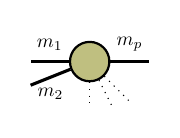
\begin{tikzpicture}[baseline=-0.5ex]
    \tikzset{tensor/.style = {minimum size = 0.5cm,shape = circle,thick,draw=black,inner sep = 0pt}, edge/.style = {thick,line width=.4mm},every loop/.style={}}
    \def\x{6}
    \node[tensor,fill=green!50!red!50!white] (A) at (\x,0) {$\At$};
    \draw[edge] (A) -- (\x-0.75,0) node [midway,above] {\scalebox{0.7}{\dimcolor{$m_1$}}};
    \draw[edge] (A) -- (\x+0.75,0) node [midway,above] {\scalebox{0.7}{\dimcolor{$m_p$}}};;
    \draw[edge] (A) -- (\x-0.75,-0.3) node [midway, below] {\scalebox{0.7}{\dimcolor{$m_2$}}};;
    \draw[dotted] (A) -- (\x,-0.6);
    \draw[dotted] (A) -- (\x+0.5,-0.5);
    \draw[dotted] (A) -- (\x+0.3,-0.6);
    \end{tikzpicture}
\hspace{0.3cm}
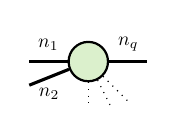
\begin{tikzpicture}[baseline=-0.5ex]
    \tikzset{tensor/.style = {minimum size = 0.5cm,shape = circle,thick,draw=black,inner sep = 0pt}, edge/.style = {thick,line width=.4mm},every loop/.style={}}
    \def\x{6}
    \def\y{0}
    \node[tensor,fill=green!70!red!20!white] (B) at (\x+1,\y) {$\Bt$};
    \draw[edge] (B) -- (\x+0.25,0) node [midway,above] {\scalebox{0.7}{\dimcolor{$n_1$}}};
    \draw[edge] (B) -- (\x+1.75,0) node [midway,above] {\scalebox{0.7}{\dimcolor{$n_q$}}};;
    \draw[edge] (B) -- (\x+0.25,-0.3) node [midway, below] {\scalebox{0.7}{\dimcolor{$n_2$}}};
    \draw[dotted] (B) -- (\x+1,-0.6);
    \draw[dotted] (B) -- (\x+1.5,-0.5);
    \draw[dotted] (B) -- (\x+1.3,-0.6);
\end{tikzpicture}\in\RR^{m_1\times\dots\times m_p\times n_1\times\dots\times n_q}.
$$
更一般地，对任意多个、阶数任意的张量，其外积的张量网络图只需把它们并排摆放即可得到。例如对  $\Tt\in\RR^{d_1\times d_2\times d_3 \times d_4}$、$\Ab\in\RR^{m\times n}$ 与 $\vb\in\RR^{p}$
$$
\Ab\outprod \Tt\outprod \vb
=
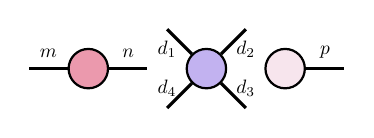
\begin{tikzpicture}[baseline=-0.5ex]
    \tikzset{tensor/.style = {minimum size = 0.5cm,shape = circle,thick,draw=black,inner sep = 0pt}, edge/.style = {thick,line width=.4mm},every loop/.style={}}
    \def\x{0}
    \def\y{0}
    \node[tensor,fill=blue!20!red!40!white] (A) at (\x,\y) {$\Ab$};
    \draw[edge] (A) -- (\x+0.75,\y)node [midway, above] {\scalebox{0.7}{\dimcolor{$n$}}};
    \draw[edge] (A) -- (\x-0.75,\y)node [midway, above] {\scalebox{0.7}{\dimcolor{$m$}}};
    \node[tensor,fill=red!20!blue!30!white] (T) at (\x+1.5,\y) {$\Tt$};
    \node[tensor,fill=red!70!blue!10!white] (v) at (\x+2.5,\y) {$\vb$};
    \draw[edge](T) -- (\x+2,\y-0.5);
    \node[draw=none] () at (\x+2,\y-0.25) {\scalebox{0.7}{\dimcolor{$d_3$}}};
    \draw[edge](T) -- (\x+2,\y+0.5);
    \node[draw=none] () at (\x+2,\y+0.25) {\scalebox{0.7}{\dimcolor{$d_2$}}};
    \draw[edge](T) -- (\x+1,\y-0.5);
    \node[draw=none] () at (\x+1,\y-0.25) {\scalebox{0.7}{\dimcolor{$d_4$}}};
    \draw[edge](T) -- (\x+1,\y+0.5);
    \node[draw=none] () at (\x+1,\y+0.25) {\scalebox{0.7}{\dimcolor{$d_1$}}};
    \draw[edge](v) -- (\x+3.25,\y)node [midway, above] {\scalebox{0.7}{\dimcolor{$p$}}};
\end{tikzpicture}\in\RR^{m\times n \times d_1\times d_2\times d_3 \times d_4\times p},
$$
其逐元素定义为 $(\Ab\outprod\Tt\outprod \vb)_{i_1i_2j_1j_2j_3j_4k} = \Ab_{i_1i_2}\Tt_{j_1\cdots j_4}\vb_{k}$，其中对 $l\in[4]$ 有 $i_1\in[m],i_2\in[n],j_l\in[d_l]$，且 $k\in[p]$。

下面的命题给出一个简洁的图示证明：外积的内积等于内积的乘积。
\begin{proposition}
    设 $\Xt,\Tt\in\RR^{d_1\times d_2\times\cdots\times d_N}$，其中 $\Xt = \ab_1\outprod\ab_2\outprod\cdots\outprod\ab_N$、$\Tt = \tb_1\outprod\tb_2\outprod\cdots\outprod\tb_N$，则 $\langle\Xt,\Tt\rangle = \prod_{n=1}^N\langle\ab_n,\tb_n\rangle$。
\begin{proof}
\begin{align*}
\langle\Xt,\Tt\rangle
&=
\left\langle\begin{tikzpicture}[baseline=\baseline]
    \tikzset{tensor/.style = {minimum size = 0.5cm,shape = circle,thick,draw=black,inner sep = 0pt}, edge/.style   = {thick,line width=.4mm}}
    \def\y{0}
     \def\x{0}
\node[tensor,fill=blue!10!white] (a1) at (\x,\y){$\ab_1$};
\node[tensor,fill=blue!10!white](a2) at (\x+1,\y){$\ab_2$};
  \node[tensor,fill=blue!10!white](an) at (\x+3,\y){$\ab_N$};
    \draw[edge] (a1) -- (\x,\y-0.7) node [midway, left] {\scalebox{0.7}{\dimcolor{$d_1$}}};
    \draw[edge] (a2) -- (\x+1,\y-0.7) node [midway, left] {\scalebox{0.7}{\dimcolor{$d_2$}}};
    \draw[edge] (an) -- (\x+3,\y-0.7)  node [midway, left] {\scalebox{0.7}{\dimcolor{$d_N$}}};
    \node (eq) at (\x+2,\y) {$\cdots$};
\end{tikzpicture} \ \scalebox{1.5}{,}
\begin{tikzpicture}[baseline=\baseline]
    \tikzset{tensor/.style = {minimum size = 0.5cm,shape = circle,thick,draw=black,inner sep = 0pt}, edge/.style   = {thick,line width=.4mm}}
    \def\y{0}
     \def\x{0}
\node[tensor,fill=red!10!white] (t1) at (\x,\y){$\tb_1$};
\node[tensor,fill=red!10!white](t2) at (\x+1,\y){$\tb_2$};
  \node[tensor,fill=red!10!white](tn) at (\x+3,\y){$\tb_N$};
    \draw[edge] (t1) -- (\x,\y-0.7) node [midway, left] {\scalebox{0.7}{\dimcolor{$d_1$}}};
    \draw[edge] (t2) -- (\x+1,\y-0.7) node [midway, left] {\scalebox{0.7}{\dimcolor{$d_2$}}};
    \draw[edge] (tn) -- (\x+3,\y-0.7)  node [midway, left] {\scalebox{0.7}{\dimcolor{$d_N$}}};
    \node (eq) at (\x+2,\y) {$\cdots$};
\end{tikzpicture} 
\right\rangle\\
&=
\begin{tikzpicture}[baseline=\baseline]
    \tikzset{tensor/.style = {minimum size = 0.5cm,shape = circle,thick,draw=black,inner sep = 0pt}, edge/.style   = {thick,line width=.4mm}}
    \def\y{0}
     \def\x{0}
\node[tensor,fill=blue!10!white] (a1) at (\x,\y+0.5){$\ab_1$};
\node[tensor,fill=blue!10!white](a2) at (\x+1,\y+0.5){$\ab_2$};
  \node[tensor,fill=blue!10!white](an) at (\x+3,\y+0.5){$\ab_N$};
  \node[tensor,fill=red!10!white] (t1) at (\x,\y-0.5){$\tb_1$};
\node[tensor,fill=red!10!white](t2) at (\x+1,\y-0.5){$\tb_2$};
  \node[tensor,fill=red!10!white](tn) at (\x+3,\y-0.5){$\tb_N$};
    \draw[edge] (a1) -- (t1) node [midway, left] {\scalebox{0.7}{\dimcolor{$d_1$}}};
    \draw[edge] (a2) -- (t2) node [midway, left] {\scalebox{0.7}{\dimcolor{$d_2$}}};
    \draw[edge] (an) -- (tn)  node [midway, left] {\scalebox{0.7}{\dimcolor{$d_N$}}};
    \node (eq) at (\x+2,\y) {$\cdots$};
\end{tikzpicture}
=
\prod_{n=1}^N\langle\ab_n,\tb_n\rangle.
\end{align*}
\end{proof}
\end{proposition}
\paragraph{维度为 1 的边等于没有边}
需要注意，在张量网络图中，大小为 1 的边等价于没有这条边。
例如在矩阵乘法中，若收缩边的大小为 1，它就等价于向量的外积：
\begin{align*}
    \Ab\in\RR^{p\times 1},\ \ \ \Bb\in\RR^{1\times q}, \ \ \ 
(\Ab\Bb)_{ij} 
&=
\begin{tikzpicture}[baseline=\baseline]
   \tikzset{tensor/.style = {minimum size = 0.5cm,shape = circle,thick,draw=black,inner sep = 0pt}, edge/.style = {thick,line width=.4mm},every loop/.style={}}
    \def\y{0}
    \def\x{0}
    \node[tensor,fill=red!50!white] (A) at (\x,\y){\scalebox{0.85}{$\Ab$}};
    \node[tensor,fill=blue!50!white] (B) at (\x+1,\y){\scalebox{0.85}{$\Bb$}};
    \draw[edge] (A) -- (B) node [above,midway] {\scalebox{0.7}{\dimcolor{$1$}}};
    \draw[edge] (\x-0.25,\y) -- (\x-0.75,\y)  node [pos=1.3] {\scalebox{0.7}{\indcolor{$i$}}};
    \draw[edge] (\x+1.25,\y) -- (\x+1.75,\y)  node [pos=1.3] {\scalebox{0.7}{\indcolor{$j$}}};
\end{tikzpicture}\\
&=
\sum_{k=1}^{1}\Ab_{i1}\Bb_{1j}
=
\begin{tikzpicture}[baseline=\baseline]
   \tikzset{tensor/.style = {minimum size = 0.5cm,shape = circle,thick,draw=black,inner sep = 0pt}, edge/.style = {thick,line width=.4mm},every loop/.style={}}
    \def\y{0}
    \def\x{0}
    \node[tensor,fill=red!50!white] (A) at (\x,\y){\scalebox{0.85}{$\ab$}};
    \node[tensor,fill=blue!50!white] (B) at (\x+1,\y){\scalebox{0.85}{$\bb$}};
    \draw[edge] (\x-0.25,\y) -- (\x-0.75,\y)  node[pos=1.3] {\scalebox{0.7}{\indcolor{$i$}}};
    \draw[edge] (\x+1.25,\y) -- (\x+1.75,\y)  node [pos=1.3] {\scalebox{0.7}{\indcolor{$j$}}};
\end{tikzpicture}\\
&=
(\ab\outprod\bb)_{ij},
\end{align*}
其中 $\ab$ 是 $\Ab$ 的唯一一列，$\bb$ 是 $\Bb$ 的唯一一行。
\paragraph{迹} 迹运算是张量收缩作用于方阵时的特例。在张量网络中，迹自然地由一条连接矩阵两条腿的环路~（自环边）表示：
\begin{align*}
\Ab\in\RR^{d \times d},\hspace{0.5cm}
\tr(\Ab) = \sum_{i=1}^d\Ab_{ii} = \hspace*{-0.5cm}
\begin{tikzpicture}[baseline=\baseline]
   \tikzset{tensor/.style = {minimum size = 0.5cm,shape = circle,thick,draw=black,inner sep = 0pt}, edge/.style = {thick,line width=.4mm},every loop/.style={}}
    \def\y{0}
    \def\x{0}
    \node[tensor,fill=red!50!white] (A) at (\x,\y){\scalebox{0.85}{$\Ab$}};
    \draw[edge] (A) to [out=20,in=160, distance=1cm] (A);
    \node[draw=none] () at (\x,\y+0.5) {\scalebox{0.7}{\dimcolor{$d$}}};
    \end{tikzpicture}\hspace*{-0.5cm}.
\end{align*}
图中没有自由腿，这与迹是标量这一事实相吻合。张量网络图为迹在循环置换下的不变性提供了一个极为简单的证明。先从两个矩阵乘积的迹入手，设 $\Ab \in \RR^{d\times R}$、$\Bb \in \RR^{R\times d}$。  如前所述，画张量网络图时重要的只是图的结构。由此即可看出
\begin{align*}
\tr(\Ab\Bb)= 
\hspace{-0.5cm}
\begin{tikzpicture}[baseline=\baseline]
   \tikzset{tensor/.style = {minimum size = 0.5cm,shape = circle,thick,draw=black,inner sep = 0pt}, edge/.style = {thick,line width=.4mm},every loop/.style={}}
    \def\y{0}
    \def\x{0}
    \node[tensor,fill=red!50!white] (A) at (\x,\y){\scalebox{0.85}{$\Ab$}};
    \node[tensor,fill=blue!50!white] (B) at (\x+1,\y){\scalebox{0.85}{$\Bb$}};
    \draw[edge] (A) -- (B) node [midway,above]{\scalebox{0.7}{\dimcolor{$R$}}};
    \draw[edge] (A) to [out=155,in=25, distance=1cm] (B);
    \node[draw=none] () at (\x+0.5,\y+0.65) {\scalebox{0.7}{\dimcolor{$d$}}};
    \end{tikzpicture}
\hspace{-0.5cm} = 
\begin{tikzpicture}[baseline=\baseline]
   \tikzset{tensor/.style = {minimum size = 0.5cm,shape = circle,thick,draw=black,inner sep = 0pt}, edge/.style = {thick,line width=.4mm},every loop/.style={}}
    \def\y{0}
    \def\x{0}
    \node[tensor,fill=red!50!white] (A) at (\x,\y-0.5){\scalebox{0.85}{$\Ab$}};
    \node[tensor,fill=blue!50!white] (B) at (\x,\y+0.5){\scalebox{0.85}{$\Bb$}};
    \draw[edge] (A) to [out=180,in=180, distance=0.5cm] (B);
    \draw[edge] (A) to [out=0,in=0, distance=0.5cm] (B);
    \node[draw=none] () at (\x+0.8,\y) {\scalebox{0.7}{\dimcolor{$R$}}};
    \node[draw=none] () at (\x-0.8,\y) {\scalebox{0.7}{\dimcolor{$d$}}};
    \end{tikzpicture}
 =\hspace{-0.5cm}
\begin{tikzpicture}[baseline=\baseline]
   \tikzset{tensor/.style = {minimum size = 0.5cm,shape = circle,thick,draw=black,inner sep = 0pt}, edge/.style = {thick,line width=.4mm},every loop/.style={}}
    \def\y{0}
    \def\x{0}
    \node[tensor,fill=blue!50!white] (B) at (\x,\y){\scalebox{0.85}{$\Bb$}};
    \node[tensor,fill=red!50!white] (A) at (\x+1,\y){\scalebox{0.85}{$\Ab$}};
    \draw[edge] (A) -- (B)node [midway,above]{\scalebox{0.7}{\dimcolor{$R$}}};;
    \draw[edge] (B) to [out=155,in=25, distance=1cm] (A);
    \node[draw=none] () at (\x+0.5,\y+0.65) {\scalebox{0.7}{\dimcolor{$d$}}};
    \end{tikzpicture}
\hspace{-0.4cm} =
\tr(\Bb\Ab),
\end{align*}
对三个矩阵 $\Ab\in\RR^{m\times n}, \Bb\in\RR^{n\times p},  \Cb\in\RR^{p\times m}$ 也有类似结论
\begin{align*}
\tr(\Ab\Bb\Cb) = 
\hspace{-0.7cm}
\begin{tikzpicture}[baseline=\baseline]
   \tikzset{tensor/.style = {minimum size = 0.5cm,shape = circle,thick,draw=black,inner sep = 0pt}, edge/.style = {thick,line width=.4mm},every loop/.style={}}
    \def\y{0}
    \def\x{0}
    \node[tensor,fill=red!50!white] (A) at (\x,\y){\scalebox{0.85}{$\Ab$}};
    \node[tensor,fill=blue!50!white] (B) at (\x+1,\y){\scalebox{0.85}{$\Bb$}};
    \node[tensor,fill=red!30!white] (C) at (\x+2,\y){\scalebox{0.85}{$\Cb$}};
    \draw[edge] (A) -- (B) node [midway,above]{\scalebox{0.7}{\dimcolor{$n$}}};
    \draw[edge] (B) -- (C) node [midway,above]{\scalebox{0.7}{\dimcolor{$p$}}};;
    \draw[edge] (A) to [out=155,in=25, distance=1cm] (C);
    \node[draw=none] () at (\x+1,\y+0.65) {\scalebox{0.7}{\dimcolor{$m$}}};
    \end{tikzpicture}
\hspace{-0.7cm}  = 
\begin{tikzpicture}[baseline=\baseline]
   \tikzset{tensor/.style = {minimum size = 0.5cm,shape = circle,thick,draw=black,inner sep = 0pt}, edge/.style = {thick,line width=.4mm},every loop/.style={}}
    \def\y{0}
    \def\x{0}
    \node[tensor,fill=red!50!white] (A) at (\x,\y+0.5){\scalebox{0.85}{$\Ab$}};
    \node[tensor,fill=blue!50!white] (B) at (\x-0.5,\y-0.3){\scalebox{0.85}{$\Bb$}};
    \node[tensor,fill=red!30!white] (C) at (\x+0.5,\y-0.3){\scalebox{0.85}{$\Cb$}};
    \draw[edge] (A) to [out=210,in=90] (B);
    \draw[edge] (A) to [out=-30,in=90] (C);
    \draw[edge] (B) to [out=300,in=240] (C);
    \node[draw=none] () at (\x+0.55,\y+0.3) {\scalebox{0.7}{\dimcolor{$m$}}};
    \node[draw=none] () at (\x-0.55,\y+0.3) {\scalebox{0.7}{\dimcolor{$n$}}};
    \node[draw=none] () at (\x,\y-0.85) {\scalebox{0.7}{\dimcolor{$p$}}};
    \end{tikzpicture}
= 
\hspace{-0.7cm}
\begin{tikzpicture}[baseline=\baseline]
   \tikzset{tensor/.style = {minimum size = 0.5cm,shape = circle,thick,draw=black,inner sep = 0pt}, edge/.style = {thick,line width=.4mm},every loop/.style={}}
    \def\y{0}
    \def\x{0}
    \node[tensor,fill=red!30!white] (C) at (\x,\y){\scalebox{0.85}{$\Cb$}};
    \node[tensor,fill=red!50!white] (A) at (\x+1,\y){\scalebox{0.85}{$\Ab$}};
    \node[tensor,fill=blue!50!white] (B) at (\x+2,\y){\scalebox{0.85}{$\Bb$}};
    \draw[edge] (C) -- (A) node [midway,above]{\scalebox{0.7}{\dimcolor{$m$}}};
    \draw[edge] (A) -- (B) node [midway,above]{\scalebox{0.7}{\dimcolor{$n$}}};
    \draw[edge] (C) to [out=155,in=25, distance=1cm] (B);
    \node[draw=none] () at (\x+1,\y+0.65) {\scalebox{0.7}{\dimcolor{$p$}}};
    \end{tikzpicture}
\hspace{-0.7cm} = \tr(\Cb\Ab\Bb).
\end{align*}
需要注意的是，张量网络图之间的这些等式是平凡的：我们只是挪动了节点的位置，而没有改变底层图的结构。因此，这只是对同一张图的两种解读，却得到了 $\tr(\Ab\Bb\Cb)$ 与 $\tr(\Cb\Ab\Bb)$ 之间并不那么平凡的等式。

\paragraph{偏迹} \emph{偏迹}（partial trace）是一类常见运算，尤其在多体量子系统的建模中：对整个系统的密度矩阵施加偏迹，便得到系统某一部分的密度矩阵。不必深究量子系统的具体细节，只需考虑一个维度为 $d_1d_2\times d_1d_2$ 的方阵，我们把它解释为一个四阶张量 \begin{tikzpicture}[baseline=-0.5ex]
    \tikzset{tensor/.style = {minimum width = 0.8cm,minimum height = 0.4cm,shape = rounded rectangle,thick,draw=black,inner sep = 0pt}, edge/.style = {thick,line width=.4mm},every loop/.style={}}
    \def\x{0}
    \def\y{0}
    \draw[edge] (\x-0.2,\y-0.15) -- (\x-0.2,\y-0.5)node [midway,left=-0.05cm] {\scalebox{0.7}{\dimcolor{$d_1$}}};
    \draw[edge] (\x+0.2,\y-0.15) -- (\x+0.2,\y-0.5)node [midway,right=-0.05cm] {\scalebox{0.7}{\dimcolor{$d_2$}}};
    \draw[edge] (\x-0.2,\y+0.15) -- (\x-0.2,\y+0.5)node [midway,left=-0.05cm] {\scalebox{0.7}{\dimcolor{$d_1$}}};
    \draw[edge] (\x+0.2,\y+0.15) -- (\x+0.2,\y+0.5)node [midway,right=-0.05cm] {\scalebox{0.7}{\dimcolor{$d_2$}}};
    \node[tensor,fill=yellow] (Bt) at (\x,\y){$\Tt$};
    \end{tikzpicture}。
$\Tt$ 关于子空间 $\mathbb R^{d_1}$ 的偏迹是一个 $d_2\times d_2$ 矩阵，把对应的两条腿相连，即对 $d_1$ 这一维``求迹''而得到： \begin{tikzpicture}[baseline=-0.5ex]
    \tikzset{tensor/.style = {minimum width = 0.6cm,minimum height = 0.4cm,shape = rounded rectangle,thick,draw=black,inner sep = 0pt}, edge/.style = {thick,line width=.4mm},every loop/.style={}}
    \def\x{0}
    \def\y{0}
    \draw[edge] (\x-0.2,\y-0.15) -- (\x-0.2,\y-0.4);
    \draw[edge] (\x+0.2,\y-0.15) -- (\x+0.2,\y-0.5)node [midway,right=-0.05cm] {\scalebox{0.7}{\dimcolor{$d_2$}}};
    \draw[edge] (\x-0.2,\y+0.15) -- (\x-0.2,\y+0.4);
    \draw[edge] (\x+0.2,\y+0.15) -- (\x+0.2,\y+0.5)node [midway,right=-0.05cm] {\scalebox{0.7}{\dimcolor{$d_2$}}};
    \draw[edge] (\x-0.2,\y-0.39) to [out=200,in=160] (\x-0.2,\y+0.39) node [midway,left=0.35cm] {\scalebox{0.7}{\dimcolor{$d_1$}}};
    \node[tensor,fill=yellow] (Bt) at (\x,\y){$\Tt$};
    \end{tikzpicture}。类似地，$\Tt$ 关于子空间 $\mathbb R^{d_2}$ 的偏迹是 $d_1\times d_1$ 矩阵
\begin{tikzpicture}[baseline=-0.5ex]
    \tikzset{tensor/.style = {minimum width = 0.6cm,minimum height = 0.4cm,shape = rounded rectangle,thick,draw=black,inner sep = 0pt}, edge/.style = {thick,line width=.4mm},every loop/.style={}}
    \def\x{0}
    \def\y{0}
    \draw[edge] (\x-0.2,\y-0.15) -- (\x-0.2,\y-0.5)node [midway,left=-0.05cm] {\scalebox{0.7}{\dimcolor{$d_1$}}};
    \draw[edge] (\x+0.2,\y-0.15) -- (\x+0.2,\y-0.4);
    \draw[edge] (\x-0.2,\y+0.15) -- (\x-0.2,\y+0.5)node [midway,left=-0.05cm] {\scalebox{0.7}{\dimcolor{$d_1$}}};
    \draw[edge] (\x+0.2,\y+0.15) -- (\x+0.2,\y+0.4);
    \draw[edge] (\x+0.2,\y-0.39) to [out=330,in=30] (\x+0.2,\y+0.39) node [midway,right=0.3cm] {\scalebox{0.7}{\dimcolor{$d_2$}}};
    \node[tensor,fill=yellow] (Bt) at (\x,\y){$\Tt$};
\end{tikzpicture}。

\paragraph{张量的 Frobenius 范数} 张量 $\At\in\RR^{d_1\times\cdots\times d_N}$ 的 Frobenius 范数是其各元素
平方之和的平方根~（即与自身内积的平方根）。在张量网络中，三阶张量 $\At\in\RR^{d_1\times d_2\times d_3}$ 的范数表示为
\begin{align*}
\norm{\At}_F^2 = \langle\At,\At\rangle = 
\sum_{i_1=1}^{d_1}\sum_{i_2=1}^{d_2}\sum_{i_3=1}^{d_3}\At_{i_1i_2i_3}^2
=
\begin{tikzpicture}[baseline=\baseline]
    \tikzset{tensor/.style = {minimum size = 0.5cm,shape = circle,thick,draw=black,inner sep = 0pt}, edge/.style = {thick,line width=.4mm},every loop/.style={}}
    \def\y{0}
    \def\x{0}
    \node[tensor,fill=green!50!red!50!white] (At) at (\x,\y){\scalebox{0.85}{$\At$}};
    \node[tensor,fill=green!50!red!50!white] (At1) at (\x+1,\y){\scalebox{0.85}{$\At$}};
    \draw[edge] (At) -- (At1);
    \draw[edge] (At) to [out=45,in=135] (At1);
    \draw[edge] (At) to [out=-45,in=-135] (At1);
    \node[draw=none] () at (\x+0.5,\y+0.6) {\scalebox{0.7}{\dimcolor{$d_1$}}};
    \node[draw=none] () at (\x+0.5,\y+0.15) {\scalebox{0.7}{\dimcolor{$d_2$}}};
    \node[draw=none] () at (\x+0.5,\y-0.5) {\scalebox{0.7}{\dimcolor{$d_3$}}};
\end{tikzpicture} .
\end{align*}
它是矩阵 Frobenius 范数最直接、自然的推广：
\begin{align*}
 \norm{\Ab}_F^2 = \tr(\Ab\Ab^\ts) = \tr(\Ab^\ts\Ab) =  \hspace*{-0.5cm}
\begin{tikzpicture}[baseline=\baseline]
   \tikzset{tensor/.style = {minimum size = 0.5cm,shape = circle,thick,draw=black,inner sep = 0pt}, edge/.style = {thick,line width=.4mm},every loop/.style={}}
    \def\y{0}
    \def\x{0}
    \node[tensor,fill=red!50!white] (A) at (\x,\y){\scalebox{0.85}{$\Ab$}};
    \node[tensor,fill=red!50!white] (B) at (\x+1,\y){\scalebox{0.85}{$\Ab$}};
    \draw[edge] (A) -- (B) node [midway,above]{\scalebox{0.7}{\dimcolor{$n$}}};
    \draw[edge] (A) to [out=155,in=25, distance=1cm] (B);
    \node[draw=none] () at (\x+0.5,\y+0.65) {\scalebox{0.7}{\dimcolor{$m$}}};
    \end{tikzpicture} \hspace*{-0.5cm}.
\end{align*}


\paragraph{外积的 Frobenius 范数} 借助张量网络，几乎可以显然地验证：外积的 Frobenius 范数等于各因子 Frobenius 范数的乘积。例如，取 $\Ab\in\RR^{m\times n}$ 与 $\Tt\in\RR^{d_1\times d_2\times d_3}$，有
$$ \begin{tikzpicture}[baseline=-0.5ex]
    \tikzset{tensor/.style = {minimum width = 1.8cm,minimum height = 0.4cm,shape = rounded rectangle,thick,draw=black,inner sep = 0pt}, edge/.style = {thick,line width=.4mm},every loop/.style={}}
    \def\x{0}
    \def\y{0}
    \draw[edge] (\x-0.7,\y-0.15) -- (\x-0.7,\y-0.5)node [midway,left=-0.05cm] {\scalebox{0.7}{\dimcolor{$m$}}};
    \draw[edge] (\x-0.35,\y-0.15) -- (\x-0.35,\y-0.5)node [midway,left=-0.05cm] {\scalebox{0.7}{\dimcolor{$n$}}};
    \draw[edge] (\x,\y-0.15) -- (\x,\y-0.5)node [midway,left=-0.1cm] {\scalebox{0.7}{\dimcolor{$d_1$}}};
    \draw[edge] (\x+0.35,\y-0.15) -- (\x+0.35,\y-0.5)node [midway,left=-0.1cm] {\scalebox{0.7}{\dimcolor{$d_2$}}};
    \draw[edge] (\x+0.7,\y-0.15) -- (\x+0.7,\y-0.5)node [midway,left=-0.1cm] {\scalebox{0.7}{\dimcolor{$d_3$}}};
    \node[tensor,fill=yellow] (Bt) at (\x,\y){$\Ab \outprod \Tt$};
    \end{tikzpicture}
    = 
    \begin{tikzpicture}[baseline=\baseline]
   \tikzset{tensor/.style = {minimum width = 0.8cm,minimum height = 0.4cm,shape = rounded rectangle,thick,draw=black,inner sep = 0pt}, edge/.style = {thick,line width=.4mm},every loop/.style={}}
    \def\y{0}
    \def\x{0}
    \draw[edge] (\x+0.2,\y-0.15) -- (\x+0.2,\y-0.5) node [midway,left=-0.05cm]{\scalebox{0.7}{\dimcolor{$n$}}};
    \draw[edge] (\x-0.2,\y-0.15) -- (\x-0.2,\y-0.5) node [midway,left=-0.05cm]{\scalebox{0.7}{\dimcolor{$m$}}};
    \node[tensor,fill=red!50!white] (A) at (\x,\y){{$\Ab$}};

   
    \def\y{0}
    \def\x{1}
    \draw[edge] (\x-0.3,\y-0.15) -- (\x-0.3,\y-0.5) node [midway,left=-0.1cm]{\scalebox{0.7}{\dimcolor{$d_1$}}};
    \draw[edge] (\x+0.05,\y-0.15) -- (\x+0.05,\y-0.5) node [midway,left=-0.1cm]{\scalebox{0.7}{\dimcolor{$d_2$}}};
    \draw[edge] (\x+0.3,\y-0.15) -- (\x+0.3,\y-0.5) node [midway,right=-0.05cm]{\scalebox{0.7}{\dimcolor{$d_3$}}};
    \node[tensor,fill=red!30!blue!20!white] (T) at (\x,\y){{$\Tt$}};
\end{tikzpicture}
    $$
于是
\begin{align*}
\norm{\Ab\outprod\Tt}_F^2
=
\norm{
\begin{tikzpicture}[baseline=\baseline]
\tikzset{tensor/.style = {minimum width = 1.8cm,minimum height = 0.4cm,shape = rounded rectangle,thick,draw=black,inner sep = 0pt}, edge/.style = {thick,line width=.4mm},every loop/.style={}}
    \def\x{0}
    \def\y{0}
    \draw[edge] (\x-0.7,\y-0.15) -- (\x-0.7,\y-0.5)node [midway,left=-0.05cm] {\scalebox{0.7}{\dimcolor{$m$}}};
    \draw[edge] (\x-0.35,\y-0.15) -- (\x-0.35,\y-0.5)node [midway,left=-0.05cm] {\scalebox{0.7}{\dimcolor{$n$}}};
    \draw[edge] (\x,\y-0.15) -- (\x,\y-0.5)node [midway,left=-0.1cm] {\scalebox{0.7}{\dimcolor{$d_1$}}};
    \draw[edge] (\x+0.35,\y-0.15) -- (\x+0.35,\y-0.5)node [midway,left=-0.1cm] {\scalebox{0.7}{\dimcolor{$d_2$}}};
    \draw[edge] (\x+0.7,\y-0.15) -- (\x+0.7,\y-0.5)node [midway,left=-0.1cm] {\scalebox{0.7}{\dimcolor{$d_3$}}};
    \node[tensor,fill=yellow] (Bt) at (\x,\y){$\Ab \outprod \Tt$};
\end{tikzpicture}
}_F^2
=
\begin{tikzpicture}[baseline=\baseline]
\tikzset{tensor/.style = {minimum width = 1.8cm,minimum height = 0.4cm,shape = rounded rectangle,thick,draw=black,inner sep = 0pt}, edge/.style = {thick,line width=.4mm},every loop/.style={}}
    \def\x{0}
    \def\y{0.35}
    \draw[edge] (\x-0.7,\y-0.15) -- (\x-0.7,\y-0.5)node [midway,left=-0.05cm] {\scalebox{0.7}{\dimcolor{$m$}}};
    \draw[edge] (\x-0.35,\y-0.15) -- (\x-0.35,\y-0.5)node [midway,left=-0.05cm] {\scalebox{0.7}{\dimcolor{$n$}}};
    \draw[edge] (\x,\y-0.15) -- (\x,\y-0.5)node [midway,left=-0.1cm] {\scalebox{0.7}{\dimcolor{$d_1$}}};
    \draw[edge] (\x+0.35,\y-0.15) -- (\x+0.35,\y-0.5)node [midway,left=-0.1cm] {\scalebox{0.7}{\dimcolor{$d_2$}}};
    \draw[edge] (\x+0.7,\y-0.15) -- (\x+0.7,\y-0.5)node [midway,left=-0.1cm] {\scalebox{0.7}{\dimcolor{$d_3$}}};
    \node[tensor,fill=yellow] (Bt) at (\x,\y){$\Ab \outprod \Tt$};
    \node[tensor,fill=yellow] (Bt) at (\x,\y-0.7){$\Ab \outprod \Tt$};
\end{tikzpicture}
=
\begin{tikzpicture}[baseline=\baseline]
   \tikzset{tensor/.style = {minimum width = 0.9cm,minimum height = 0.4cm,shape = rounded rectangle,thick,draw=black,inner sep = 0pt}, edge/.style = {thick,line width=.4mm},every loop/.style={}}
    \def\y{0.35}
    \def\x{0}
    \draw[edge] (\x+0.2,\y-0.15) -- (\x+0.2,\y-0.5) node [midway,left=-0.05cm]{\scalebox{0.7}{\dimcolor{$n$}}};
    \draw[edge] (\x-0.2,\y-0.15) -- (\x-0.2,\y-0.5) node [midway,left=-0.05cm]{\scalebox{0.7}{\dimcolor{$m$}}};
    \node[tensor,fill=red!50!white] (A) at (\x,\y){{$\Ab$}};
    \node[tensor,fill=red!50!white] (A) at (\x,\y-0.7){{$\Ab$}};
    \def\x{1}
    \draw[edge] (\x-0.3,\y-0.15) -- (\x-0.3,\y-0.5) node [midway,left=-0.1cm]{\scalebox{0.7}{\dimcolor{$d_1$}}};
    \draw[edge] (\x+0.05,\y-0.15) -- (\x+0.05,\y-0.5) node [midway,left=-0.1cm]{\scalebox{0.7}{\dimcolor{$d_2$}}};
    \draw[edge] (\x+0.3,\y-0.15) -- (\x+0.3,\y-0.5) node [midway,right=-0.1cm]{\scalebox{0.7}{\dimcolor{$d_3$}}};
    \node[tensor,fill=red!30!blue!20!white] (T) at (\x,\y){{$\Tt$}};
    \node[tensor,fill=red!30!blue!20!white] (T) at (\x,\y-0.7){{$\Tt$}};
\end{tikzpicture}
=\norm{\Ab}_F^2 \norm{\Tt}_F^2
.
\end{align*}


\paragraph{例} 本节以最后一个例子收尾，说明张量网络的图示记法在表示复杂的张量运算时多么有用：
\begin{align}\label{eq:einsum}
\begin{tikzpicture}[baseline = \baseline]
    \tikzset{tensor/.style = {minimum size = 0.5cm,shape = circle,thick,draw=black,inner sep = 0pt}, edge/.style = 
    {thick,line width=.4mm},every loop/.style={}}
    \def\y{-0.5}
    \def\x{0}
    \node[tensor,fill=green!50!red!50!white] (At) at (\x,\y){\scalebox{0.85}{$\At$}};
    \node[tensor,fill=red!20!white] (S) at (\x-1,\y){\scalebox{0.85}{$\St$}};
    \node[tensor,fill=red!50!white] (Tt) at (\x,\y+1){\scalebox{0.85}{$\Tt$}};
    \node[tensor,fill=blue!40!red!60!white] (A) at (\x+1,\y){\scalebox{0.85}{$\Ab$}};
    \draw[edge] (Tt) -- (At) node [midway,left] {\scalebox{0.7}{\dimcolor{$R$}}};
    \draw[edge] (Tt) -- (A) node [above,midway] {\scalebox{0.7}{\dimcolor{$R$}}};
    \draw[edge] (At) -- (A)  node [midway,above] {\scalebox{0.7}{\dimcolor{$R$}}};
    \draw[edge] (Tt) -- (\x,\y+1.75) node [pos=1.3] {\scalebox{0.7}{\indcolor{$k$}}};
    \draw[edge] (At) -- (S)  node [midway,above] {\scalebox{0.7}{\dimcolor{$R$}}};
    \draw[edge] (S) -- (Tt)  node [midway,above] {\scalebox{0.7}{\dimcolor{$R$}}};
    \draw[edge] (Tt) -- (\x-0.75,\y+1)  node [pos=1.3] {\scalebox{0.7}{\indcolor{$j$}}};
    \draw[edge] (Tt) -- (\x+0.75,\y+1)  node [pos=1.3] {\scalebox{0.7}{\indcolor{$l$}}};
    \draw[edge] (S) -- (\x-1.2,\y+0.75)  node [pos=1.3] {\scalebox{0.7}{\indcolor{$i$}}};
    \end{tikzpicture}
&=
\sum_{r_1=1}^R\sum_{r_2=1}^R\sum_{r_3=1}^R\sum_{r_4=1}^R\sum_{r_5=1}^R\St_{ir_1 r_2}\At_{r_2r_3r_5}\Tt_{iklr_1r_3r_4}\Ab_{r_4r_5}\nonumber\\
&=
    \begin{tikzpicture}[baseline = \baseline]
    \tikzset{tensor/.style = {minimum size = 0.5cm,shape = circle,thick,draw=black,inner sep = 0pt}, edge/.style = 
    {thick,line width=.4mm},every loop/.style={}}
    \def\y{0}
    \def\x{0}
    \node[tensor,fill=blue!50!red!30!yellow!50!white] (Ht) at (\x,\y){\scalebox{0.85}{$\Ht$}};
    \draw[edge](Ht) -- (\x,\y+0.7) node [pos=1.3] {\scalebox{0.7}{\indcolor{$j$}}};
    \draw[edge](Ht) -- (\x,\y-0.7) node [pos=1.3] {\scalebox{0.7}{\indcolor{$l$}}};
    \draw[edge](Ht) -- (\x-0.7,\y) node [pos=1.3] {\scalebox{0.7}{\indcolor{$i$}}};
    \draw[edge](Ht) -- (\x+0.7,\y) node[pos=1.3] {\scalebox{0.7}{\indcolor{$k$}}};
    \end{tikzpicture}.
\end{align}
\subsection{复制张量~（超边）}\label{sec:copy-tensor}


有时需要表示由多于两个张量共享的同时收缩。例如，把三个向量 $\ab\in\RR^d, \bb\in\RR^d,$ 与 $\cbb\in\RR^d$ 收缩成一个标量：$\sum_{i=1}^d\ab_i\bb_i\cbb_i$。
这一运算在张量网络中可用一种特殊的张量——\emph{复制张量}（copy tensor）——来刻画。复制张量等价于克罗内克 $\delta$，也就是对角元全为 1、其余元素全为 0 的超对角张量，在张量网络图中画作一个黑点。例如，复制张量
\begin{tikzpicture}[baseline=\baseline]
   \tikzset{tensor/.style = {minimum size = 0.5cm,shape = circle,thick,draw=black,inner sep = 0pt}, edge/.style = {thick,line width=.4mm},every loop/.style={}}
    \def\y{0}
    \def\x{0}
     \draw  node[fill = black,circle,inner sep=0pt,minimum size=4pt] (m) at (\x,\y) {};
     \draw  node[draw=none] (a) at (\x-0.7,\y) {};
     \draw  node[draw=none] (b) at (\x+0.7,\y) {};
     \draw  node[draw=none] (c) at (\x,\y-0.7) {};
    \draw[edge] (a) -- (m);
    \draw[edge] (m) -- (b);
    \draw[edge] (m) -- (c);
\end{tikzpicture}
其逐元素定义为
$$
 \left(\begin{tikzpicture}[baseline=\baseline]
   \tikzset{tensor/.style = {minimum size = 0.5cm,shape = circle,thick,draw=black,inner sep = 0pt}, edge/.style = {thick,line width=.4mm},every loop/.style={}}
    \def\y{0}
    \def\x{0}
     \draw  node[fill = black,circle,inner sep=0pt,minimum size=4pt] (m) at (\x,\y) {};
     \draw  node[draw=none] (a) at (\x-0.7,\y) {};
     \draw  node[draw=none] (b) at (\x+0.7,\y) {};
     \draw  node[draw=none] (c) at (\x,\y-0.7) {};
    \draw[edge] (a) -- (m);
    \draw[edge] (m) -- (b);
    \draw[edge] (m) -- (c);
\end{tikzpicture}\right)_{ijk} = \delta_{ijk} = \begin{cases}
      1 & \text{if } i=j=k\\
      0 & \text{otherwise}
    \end{cases}.
$$
借助复制张量，上述三重收缩可表示为
\begin{align*}
\begin{tikzpicture}[baseline=\baseline]
   \tikzset{tensor/.style = {minimum size = 0.5cm,shape = circle,thick,draw=black,inner sep = 0pt}, edge/.style = {thick,line width=.4mm},every loop/.style={}}
    \def\y{0}
    \def\x{0}
    \node[tensor,fill=blue!40!red!60!white] (a) at (\x,\y){\scalebox{0.85}{$\ab$}};
    \node[tensor,fill=blue!10!white] (b) at (\x+1.5,\y){\scalebox{0.85}{$\bb$}};
    \node[tensor,fill=blue!20!red!40!white] (c) at (\x+0.7,\y-0.75){\scalebox{0.85}{$\cbb$}};
    \draw  node[fill = black,circle,inner sep=0pt,minimum size=4pt] (m) at (\x+0.7,\y) {};
    \draw[edge] (a) -- (m) node [above,midway] {\scalebox{0.7}{\dimcolor{$d$}}};
    \draw[edge] (m) -- (b) node [above,midway] {\scalebox{0.7}{\dimcolor{$d$}}};
    \draw[edge] (m) -- (c) node [left,midway] {\scalebox{0.7}{\dimcolor{$d$}}};
    \end{tikzpicture} = \sum_{i,j,k=1}^d\delta_{ijk}\ab_i\bb_j\cbb_k =
\sum_{i=1}^d\ab_i\bb_i\cbb_i .
\end{align*}
下面给出任意阶 $N$ 的复制张量更严格的定义。
\begin{definition}
阶为 N 的复制张量
   \begin{tikzpicture}[baseline=\baseline]
    \tikzset{tensor/.style = {minimum size = 0.5cm,shape = circle,thick,draw=black,inner sep = 0pt}, edge/.style   = {thick,line width=.4mm},every loop/.style={}}
    \def\y{0}
    \def\x{0}
    \draw  node[fill = black,circle,inner sep=0pt,minimum size=4pt] (m) at (\x,\y) {};
    \draw[edge] (m) -- (\x-0.6,0) node [midway,above] {\scalebox{0.7}{\dimcolor{$d$}}};
    \draw[edge] (m) -- (\x+0.6,0) node [midway,above] {\scalebox{0.7}{\dimcolor{$d$}}};;
    \draw[edge] (m) -- (\x-0.5,-0.3) node [midway, below] {\scalebox{0.7}{\dimcolor{$d$}}};;
    \draw[dotted] (m) -- (\x,-0.6);
    \draw[dotted] (m) -- (\x,-0.6);
    \draw[dotted] (m) -- (\x+0.5,-0.5);
    \draw[dotted] (m) -- (\x+0.3,-0.6);
\end{tikzpicture}
是形状为 $\underbrace{d\times d\dots\times d}_{N\text{ times}}$ 的张量，定义为
\begin{align*}
       \begin{tikzpicture}[baseline=\baseline]
    \tikzset{tensor/.style = {minimum size = 0.5cm,shape = circle,thick,draw=black,inner sep = 0pt}, edge/.style   = {thick,line width=.4mm},every loop/.style={}}
    \def\y{0}
    \def\x{0}
    \draw  node[fill = black,circle,inner sep=0pt,minimum size=4pt] (m) at (\x,\y) {};
    \draw[edge] (m) -- (\x-0.6,0) node [midway,above] {\scalebox{0.7}{\dimcolor{$d$}}};
    \draw[edge] (m) -- (\x+0.6,0) node [midway,above] {\scalebox{0.7}{\dimcolor{$d$}}};;
    \draw[edge] (m) -- (\x-0.5,-0.3) node [midway, below] {\scalebox{0.7}{\dimcolor{$d$}}};;
    \draw[dotted] (m) -- (\x,-0.6);
    \draw[dotted] (m) -- (\x,-0.6);
    \draw[dotted] (m) -- (\x+0.5,-0.5);
    \draw[dotted] (m) -- (\x+0.3,-0.6);
\end{tikzpicture}
= \sum_{i=1}^d\underbrace{\eb_i\outprod\eb_i\outprod\dots\outprod\eb_i}_{N\text{ times}},%
\end{align*}
其中 $\eb_1,\eb_2,\dots,\eb_d$ 为 $\RR^{d}$ 的标准基向量。
\end{definition}
复制张量之名正由此而来：与复制张量收缩，便可``复制''标准基向量。事实上，设 $\eb_i\in\RR^{d}$ 为标准基向量，则容易
验证
$       
\begin{tikzpicture}[baseline=\baseline]
    \tikzset{tensor/.style = {minimum size = 0.5cm,shape = circle,thick,draw=black,inner sep = 0pt}, edge/.style   = {thick,line width=.4mm},every loop/.style={}}
    \def\y{0}
    \def\x{0}
    \node[tensor,fill=blue!40!red!60!white] (e) at (\x,\y){\scalebox{0.85}{$\eb_i$}};
    \draw  node[fill = black,circle,inner sep=0pt,minimum size=4pt] (m) at (\x+0.75,\y) {};
    \draw[edge] (e) -- (m) node [midway,above] {\scalebox{0.7}{\dimcolor{$d$}}};
    \draw[edge] (m) -- (\x+1.4,\y) node [midway,above] {\scalebox{0.7}{\dimcolor{$d$}}};
    \draw[edge] (m) -- (\x+0.75,\y-0.7) node [midway,right] {\scalebox{0.7}{\dimcolor{$d$}}};
    \node[draw=none] () at (\x+2,\y) {\scalebox{1}{$=$}};
    \node[tensor,fill=blue!40!red!60!white] (e1) at (\x+2.5,\y){\scalebox{0.85}{$\eb_i$}};
    \node[tensor,fill=blue!40!red!60!white] (e2) at (\x+3.5,\y){\scalebox{0.85}{$\eb_i$}};
    \draw[edge] (e2) -- (\x+3.5,\y-0.7) node [midway,right] {\scalebox{0.7}{\textcolor{gray}{$d$}}};
    \draw[edge] (e1) -- (\x+2.5,\y-0.7) node [midway,right] {\scalebox{0.7}{\textcolor{gray}{$d$}}};
\end{tikzpicture}.
$
简短证明如下：
\begin{align*}
    \left(
\begin{tikzpicture}[baseline=\baseline]
    \tikzset{tensor/.style = {minimum size = 0.5cm,shape = circle,thick,draw=black,inner sep = 0pt}, edge/.style   = {thick,line width=.4mm},every loop/.style={}}
    \def\y{0}
    \def\x{0}
    \node[tensor,fill=blue!40!red!60!white] (e) at (\x,\y){\scalebox{0.85}{$\eb_i$}};
    \draw  node[fill = black,circle,inner sep=0pt,minimum size=4pt] (m) at (\x+0.75,\y) {};
    \draw[edge] (e) -- (m) node [midway,above] {\scalebox{0.7}{\dimcolor{$d$}}};
    \draw[edge] (m) -- (\x+1.4,\y) node [midway,above] {\scalebox{0.7}{\dimcolor{$d$}}};
    \draw[edge] (m) -- (\x+0.75,\y-0.7)node [midway,right] {\scalebox{0.7}{\dimcolor{$d$}}};
\end{tikzpicture}\right)_{jk}
&= 
\sum_{s}(\eb_i)_{s}\delta_{sjk} = \sum_{s}\delta_{is}\delta_{sjk} = \delta_{ijk}\\ 
&= 
\begin{cases}
     1 & \text{if } i=j=k\\
      0 & \text{otherwise}.
    \end{cases} =
    (\eb_i\eb_i^\ts)_{j,k} =
\begin{tikzpicture}[baseline=\baseline]
    \tikzset{tensor/.style = {minimum size = 0.5cm,shape = circle,thick,draw=black,inner sep = 0pt}, edge/.style   = {thick,line width=.4mm},every loop/.style={}}
    \def\y{0}
    \def\x{0}
    \node[tensor,fill=blue!40!red!60!white] (e1) at (\x,\y){\scalebox{0.85}{$\eb_i$}};
    \node[tensor,fill=blue!40!red!60!white] (e2) at (\x+1,\y){\scalebox{0.85}{$\eb_i$}};
    \draw[edge] (e2) -- (\x+1,\y-0.7) node [below] {\scalebox{0.7}{\indcolor{$k$}}};
    \draw[edge] (e1) -- (\x,\y-0.7) node [below] {\scalebox{0.7}{\indcolor{$j$}}};
\end{tikzpicture}.
\end{align*}
务必注意，复制张量的``复制''性质只对标准基向量成立，对任意向量并不成立：一般而言
$       
\begin{tikzpicture}[baseline=\baseline]
    \tikzset{tensor/.style = {minimum size = 0.5cm,shape = circle,thick,draw=black,inner sep = 0pt}, edge/.style   = {thick,line width=.4mm},every loop/.style={}}
    \def\y{0}
    \def\x{0}
    \node[tensor,fill=blue!40!red!60!white] (e) at (\x,\y){\scalebox{0.85}{$\vb$}};
    \draw  node[fill = black,circle,inner sep=0pt,minimum size=4pt] (m) at (\x+0.75,\y) {};
    \draw[edge] (e) -- (m) node [midway,above] {\scalebox{0.7}{\dimcolor{$d$}}};
    \draw[edge] (m) -- (\x+1.4,\y) node [midway,above] {\scalebox{0.7}{\dimcolor{$d$}}};
    \draw[edge] (m) -- (\x+0.75,\y-0.7) node [midway,right] {\scalebox{0.7}{\dimcolor{$d$}}};
    \node[draw=none] () at (\x+2,\y) {\scalebox{1}{$\neq$}};
    \node[tensor,fill=blue!40!red!60!white] (e1) at (\x+2.5,\y){\scalebox{0.85}{$\vb$}};
    \node[tensor,fill=blue!40!red!60!white] (e2) at (\x+3.5,\y){\scalebox{0.85}{$\vb$}};
    \draw[edge] (e2) -- (\x+3.5,\y-0.7) node [midway,right] {\scalebox{0.7}{\dimcolor{$d$}}};
    \draw[edge] (e1) -- (\x+2.5,\y-0.7) node [midway,right] {\scalebox{0.7}{\dimcolor{$d$}}};
\end{tikzpicture}
$。复制张量之所以只``复制''基向量，是因为 $\delta_{ijk}$ 只挑出对角元。
\begin{proposition}\label{prop:copy.tensor} 下面列出复制张量的若干有用性质。
\begin{enumerate}
    \item 最简单的复制张量是元素全为 1 的向量，即
$$
  \begin{tikzpicture}[baseline=\baseline]
    \tikzset{tensor/.style = {minimum size = 0.5cm,shape = circle,thick,draw=black,inner sep = 0pt}, edge/.style   = {thick,line width=.4mm},every loop/.style={}}
    \def\y{0.5}
    \def\x{0}
    \draw  node[fill = black,circle,inner sep=0pt,minimum size=4pt] (m) at (\x,\y) {};
    \draw[edge] (m) -- (\x,\y-1) node [left,midway] {\scalebox{0.7}{\dimcolor{$n$}}};
 \end{tikzpicture}
 =\sum_{i=1}^n\eb_i =\overrightarrow{\mathbf{1}}.
$$\label{itm:one-copy-tensor}
\item 二阶复制张量就是单位矩阵，此处可直接省去中间的黑点，把它画成一条线，即
$
    \begin{tikzpicture}[baseline=\baseline]
    \tikzset{tensor/.style = {minimum size = 0.5cm,shape = circle,thick,draw=black,inner sep = 0pt}, edge/.style   = {thick,line width=.4mm},every loop/.style={}}
    \def\y{0}
    \def\x{0}
    \draw  node[fill = black,circle,inner sep=0pt,minimum size=4pt] (m) at (\x,\y) {};
    \draw  node[fill = black,circle,inner sep=0pt,minimum size=4pt] (m) at (\x,\y) {};
    \draw[edge] (m) -- (\x-0.6,0) node [very near end,left] {\scalebox{0.7}{\indcolor{$i$}}};
    \draw[edge] (m) -- (\x+0.6,0) node [very near end,right]
    {\scalebox{0.7}{\indcolor{$i$}}};
    \node[draw=none] at (\x+1,\y) {\scalebox{1}{\textcolor{black}{$=$}}};;
    \draw[edge] (\x+1.3,\y) -- (\x+2.5,\y) node [very near start,left=0.05cm] {\scalebox{0.7}{\indcolor{$i$}}} node [very near end,right=0.05cm] {\scalebox{0.7}{\indcolor{$i$}}};
    \end{tikzpicture} = \delta_{ij} = \begin{cases}
      1 & \text{if } i=j\\
      0 & \text{otherwise},
    \end{cases}
    =
    \Ib_{ij}.
$
\item 
有趣的是，把一个复制张量的任意若干条腿与另一个复制张量的腿收缩后，所得的张量网络本身仍是一个复制
张量（在图中把被收缩的腿与黑点合并即得）。例如：
\begin{align*}  
\sum_{l_1}\delta_{i_1j_1k_1l_1}\delta_{i_2j_2k_2l_1} 
&=
\begin{tikzpicture}[baseline=\baseline]
    \tikzset{tensor/.style = {minimum size = 0.5cm,shape = circle,thick,draw=black,inner sep = 0pt}, edge/.style   = {thick,line width=.4mm},every loop/.style={}}
    \def\y{0}
    \def\x{0}
    \draw  node[fill = black,circle,inner sep=0pt,minimum size=4pt] (m) at (\x,\y) {};
    \draw[edge] (m) -- (\x,\y-0.5)node [below] {\scalebox{0.6}{\indcolor{$i_1$}}};
    \draw[edge](m) -- (\x,\y+0.5)node [above] {\scalebox{0.6}{\indcolor{$
    k_1$}}};
    \draw[edge] (m) -- (\x-0.5,\y)node [left] {\scalebox{0.6}{\indcolor{$j_1$}}};
    \draw  node[fill = black,circle,inner sep=0pt,minimum size=4pt] (n) at (\x+1,\y) {};
    \draw[edge] (n) -- (\x+1.5,\y)node [right] {\scalebox{0.6}{\indcolor{$j_2$}}};
    \draw[edge] (n) --  (\x+1,\y+0.5)node [above] {\scalebox{0.6}{\indcolor{$k_2$}}};   
    \draw[edge] (n) -- (\x+1,\y-0.5)node [below] {\scalebox{0.6}{\indcolor{$i_2$}}};
    \draw[edge](m) -- (n)node [midway, above] {\scalebox{0.6}{\indcolor{$l_1$}}};
 \end{tikzpicture}
= 
\delta_{i_1j_1k_1i_2j_2k_2}\\
&=
\begin{tikzpicture}[baseline=\baseline]
    \tikzset{tensor/.style = {minimum size = 0.5cm,shape = circle,thick,draw=black,inner sep = 0pt}, edge/.style   = {thick,line width=.4mm},every loop/.style={}}
    \def\y{0}
    \def\x{0}
    \draw node[fill = black,circle,inner sep=0pt,minimum size=5pt] (m) at (\x,\y) {};
    \draw[edge] (m) -- (\x+0.75,\y)node [right] {\scalebox{0.6}{\indcolor{$j_2$}}};
    \draw[edge] (m) -- (\x-0.75,\y)node [left] {\scalebox{0.6}{\indcolor{$j_1$}}};
    \draw[edge] (m) -- (\x+0.5,\y-0.5)node [below] {\scalebox{0.6}{\indcolor{$i_2$}}};
    \draw[edge] (m) -- (\x-0.5,\y+0.5)node [above] {\scalebox{0.6}{\indcolor{$k_1$}}};
    \draw[edge] (m) -- (\x-0.5,\y-0.5)node [below] {\scalebox{0.6}{\indcolor{$i_1$}}};
    \draw[edge] (m) -- (\x+0.5,\y+0.5)node [above] {\scalebox{0.6}{\indcolor{$k_2$}}};
\end{tikzpicture}
=
 \begin{tikzpicture}[baseline=\baseline]
    \tikzset{tensor/.style = {minimum size = 0.5cm,shape = circle,thick,draw=black,inner sep = 0pt}, edge/.style   = {thick,line width=.4mm},every loop/.style={}}
    \def\y{0}
    \def\x{0}
    \draw  node[fill = black,circle,inner sep=0pt,minimum size=5pt] (m) at (\x,\y+0.4) {};
    \draw  node[fill = black,circle,inner sep=0pt,minimum size=5pt] (n) at (\x,\y-0.4) {};
    \draw[edge] (n) -- (m)node [midway, right] {\scalebox{0.6}{\indcolor{$i_1$}}};;
    \draw[edge](m) -- (\x,\y+1)node [above] {\scalebox{0.6}{\indcolor{$k_2$}}};
    \draw[edge](n) -- (\x,\y-1)node [below] {\scalebox{0.6}{\indcolor{$k_1$}}};
    \draw[edge](m) -- (\x+0.45,\y+0.65)node [above] {\scalebox{0.6}{\indcolor{$l_2$}}};
    \draw[edge](m) -- (\x-0.45,\y+0.65)node [above] {\scalebox{0.6}{\indcolor{$j_2$}}};
    \draw[edge](n) -- (\x+0.45,\y-0.65)node [above] {\scalebox{0.6}{\indcolor{$l_1$}}};;
    \draw[edge](n) -- (\x-0.45,\y-0.65)node [above] {\scalebox{0.6}{\indcolor{$j_1$}}};;
    \end{tikzpicture}
=
\sum_{i_1}\delta_{i_1j_1k_1l_1}\delta_{i_1j_2k_2l_2}.
\end{align*}
\item\label{prop:diagcopy}
对任意向量 $\vb\in\RR^n$，记 $\diag(\vb)\in\RR^{n\times n}$ 为以 $\vb$ 的各分量作对角元的对角矩阵；对任意矩阵 $\Ab\in\RR^{n\times n}$，记 $\diag(\Ab)\in\RR^{n}$ 为取出 $\Ab\in\RR^{n\times n}$ 全部对角元所得的向量。
于是
$$
    \diag(\vb) = 
     \begin{tikzpicture}[baseline=\baseline]
    \tikzset{tensor/.style = {minimum size = 0.5cm,shape = circle,thick,draw=black,inner sep = 0pt}, edge/.style   = {thick,line width=.4mm},every loop/.style={}}
    \def\y{0}
    \def\x{0}
    \draw  node[fill = black,circle,inner sep=0pt,minimum size=4pt] (m) at (\x,\y) {};
    \node[tensor,fill=blue!20!red!40!white] (v) at (\x,\y-0.85){\scalebox{0.85}{$\vb$}};
    \draw[edge] (m) -- (\x-0.6,0);
    \draw[edge] (m) -- (\x+0.6,0);
    \draw[edge] (m) -- (\x,\y-0.6); 
    \node[draw=none] at (\x+1,\y) {\scalebox{1}{\textcolor{black}{$=$}}};
    \node[tensor,fill=blue!20!red!40!white] (v) at (\x+2.5,\y){\scalebox{0.85}{}};
    \draw[edge] (v) -- (\x+3.5,\y);
    \draw[edge] (v) -- (\x+1.5,\y);
  \draw[edge=0.5] (v.south west) -- (v.north east);
\end{tikzpicture} 
~~\text{and}~~
\diag(\Ab) =\hspace{-0.7cm}
\begin{tikzpicture}[baseline=\baseline]
    \tikzset{tensor/.style = {minimum size = 0.5cm,shape = circle,thick,draw=black,inner sep = 0pt}, edge/.style = {thick,line width=.4mm},every loop/.style={}}
    \def\y{0}
    \def\x{0}
    \node[tensor,fill=red!50!white] (A) at (\x,\y+0.2){\scalebox{0.85}{$\Ab$}};
    \draw[edge] (A) to [out=-20,in=-160, distance=1.35cm] (A);
    \draw  node[fill = black,circle,inner sep=0pt,minimum size=4pt] (m) at (\x,\y-0.25) {};
    \draw[edge] (m) -- (\x,\y-0.65);
    \end{tikzpicture},
$$
其中
$
\begin{tikzpicture}[baseline=\baseline]
    \tikzset{tensor/.style = {minimum size = 0.5cm,shape = circle,thick,draw=black,inner sep = 0pt}, edge/.style = {thick,line width=.4mm},every loop/.style={}}
    \def\y{0}
    \def\x{0}
    \node[tensor,fill=blue!20!red!40!white] (v) at (\x+2.5,\y){\scalebox{0.85}{}};
    \draw[edge] (v) -- (\x+3.5,\y);
    \draw[edge] (v) -- (\x+1.5,\y);
  \draw[edge=0.5] (v.south west) -- (v.north east);
\end{tikzpicture} 
$ 
表示一个对角矩阵。
\begin{proof}
第一条：对任意 $i,j\in [n]$，有
\begin{align*}
    \begin{tikzpicture}[baseline=-15]
    \tikzset{tensor/.style = {minimum size = 0.5cm,shape = circle,thick,draw=black,inner sep = 0pt}, edge/.style   = {thick,line width=.4mm},every loop/.style={}}
    \def\y{0}
    \def\x{0}
    \draw  node[fill = black,circle,inner sep=0pt,minimum size=4pt] (m) at (\x,\y) {};
   \node[tensor,fill=blue!20!red!40!white] (v) at (\x,\y-0.85){\scalebox{0.85}{$\vb$}};
    \draw[edge] (m) -- (\x-0.6,0) node [very near end,left] {\scalebox{0.7}{\indcolor{$i$}}};
    \draw[edge] (m) -- (\x+0.6,0)node [very near end,right] {\scalebox{0.7}{\indcolor{$j$}}};;
    \draw[edge] (m) -- (\x,\y-0.6);
 \end{tikzpicture}
&=
 \sum_{k}
\left(\begin{tikzpicture}[baseline=-15]
    \tikzset{tensor/.style = {minimum size = 0.5cm,shape = circle,thick,draw=black,inner sep = 0pt}, edge/.style   = {thick,line width=.4mm},every loop/.style={}}
    \def\y{0}
    \def\x{0}
    \draw  node[fill = black,circle,inner sep=0pt,minimum size=4pt] (m) at (\x,\y) {};
    \draw[edge] (m) -- (\x-0.6,0)node [very near end, left] {\scalebox{0.7}{\indcolor{$i$}}};;
    \draw[edge] (m) -- (\x+0.6,0)node [very near end, right] {\scalebox{0.7}{\indcolor{$j$}}};
    \draw[edge] (m) -- (\x,\y-0.6)node [very near end, below]{\scalebox{0.7}{\indcolor{$k$}}};  \node[tensor,fill=blue!20!red!40!white] (v) at (\x+1.25,\y-0.8){\scalebox{0.85}{$\vb$}};
    \draw[edge] (v) -- (\x+1.25,0)node [very near end, above] {\scalebox{0.7}{\indcolor{$k$}}};;
 \end{tikzpicture}\right)\\
&= 
\sum_{k}\delta_{ijk}\vb_k = 
\delta_{ij}\vb_i
= 
\begin{cases}
\vb_i & \text{ if } i=j\\
0 &\text{ otherwise}
\end{cases}
= \text{diag}(\vb)_{ij}.
\end{align*}
第二条：对任意 $i\in [n]$，有
\begin{align*}
    \begin{tikzpicture}[baseline=\baseline]
    \tikzset{tensor/.style = {minimum size = 0.5cm,shape = circle,thick,draw=black,inner sep = 0pt}, edge/.style = {thick,line width=.4mm},every loop/.style={}}
    \def\y{0}
    \def\x{0}
    \node[tensor,fill=red!50!white] (A) at (\x,\y+0.2){\scalebox{0.85}{$\Ab$}};
    \draw[edge] (A) to [out=-20,in=-160, distance=1.35cm] (A);
    \draw  node[fill = black,circle,inner sep=0pt,minimum size=4pt] (m) at (\x,\y-0.25) {};
    \draw[edge] (m) -- (\x,\y-0.65)node [very near end, below] {\scalebox{0.7}{\indcolor{$i$}}};
\end{tikzpicture}\hspace{-0.7cm}
=
\sum_{j,k}\left(
\begin{tikzpicture}[baseline=\baseline]
    \tikzset{tensor/.style = {minimum size = 0.5cm,shape = circle,thick,draw=black,inner sep = 0pt}, edge/.style = {thick,line width=.4mm},every loop/.style={}}
    \def\y{0}
    \def\x{0}
    \node[tensor,fill=red!50!white] (A) at (\x,\y+0.4){\scalebox{0.85}{$\Ab$}};
    \draw  node[fill = black,circle,inner sep=0pt,minimum size=4pt] (m) at (\x,\y-0.25) {};
    \draw[edge] (m) -- (\x-0.7,\y-0.25)node [very near end,left] {\scalebox{0.7}{\indcolor{$k$}}};
    \draw[edge] (m) -- (\x+0.7,\y-0.25)node [very near end,right] {\scalebox{0.7}{\indcolor{$j$}}};
    \draw[edge] (m) -- (\x,\y-0.75)node [very near end, below] {\scalebox{0.7}{\indcolor{$i$}}};
    \draw[edge] (A) --(\x+0.7,\y+0.4)node [very near end,right] {\scalebox{0.7}{\indcolor{$j$}}};
    \draw[edge] (A) --(\x-0.7,\y+0.4)node [very near end,left] {\scalebox{0.7}{\indcolor{$k$}}};
    \end{tikzpicture}\right)
=
\sum_{j,k}\delta_{ijk}\Ab_{kj}
=
\Ab_{ii} = \diag(\Ab)
_{i}.
\end{align*}
\end{proof}
\item\label{prop:diag}
由此不难验证 $\diag(\vb)\diag(\ub)$ =
    \begin{tikzpicture}[baseline=\baseline]
    \tikzset{tensor/.style = {minimum size = 0.5cm,shape = circle,thick,draw=black,inner sep = 0pt}, edge/.style   = {thick,line width=.4mm},every loop/.style={}}
    \def\y{0}
    \def\x{0}
    \draw  node[fill = black,circle,inner sep=0pt,minimum size=4pt] (m) at (\x,\y) {};
    \node[tensor,fill=blue!20!red!40!white] (v) at (\x,\y-0.85){\scalebox{0.85}{$\vb$}};
    \draw[edge] (m) -- (\x-0.6,0);
    \draw[edge] (m) -- (\x,\y-0.6); 
    \draw  node[fill = black,circle,inner sep=0pt,minimum size=4pt] (m1) at (\x+1,\y) {};
    \node[tensor,fill=red!20!blue!40!white] (u) at (\x+1,\y-0.85){\scalebox{0.85}{$\ub$}};
    \draw[edge] (m1) -- (m);
    \draw[edge] (m1) -- (\x+1.6,0);
    \draw[edge] (m1) -- (\x+1,\y-0.6); 
\end{tikzpicture}.
\end{enumerate}
\end{proposition}

\subsection{张量网络中的矩阵分解}
与任何其他运算一样，张量分解也可以用张量网络图来描绘。本节将介绍矩阵分解的图形化图示。更高阶张量的一般分解将在第~\ref{chapter:tensor-decomposition}章中讨论。在张量网络中，分解是指把一个节点拆分为多个节点；我们称其逆运算为合并（merging），即把多个节点组合成一个节点。这一过程可以由下面的张量网络图清晰地说明：
\begin{align*}
\begin{tikzpicture}[baseline=\baseline]
    \tikzset{tensor/.style = {minimum size = 0.5cm,shape = circle,thick,draw=black,inner sep = 0pt}, edge/.style = {thick,line width=.4mm},every loop/.style={}}
    \def\y{0}
    \def\x{0}
    \node[tensor,fill=red!50!white] (A) at (\x,\y){\scalebox{0.85}{$\Ab$}};
    \node[tensor,fill=blue!50!white] (B) at (\x+2,\y){\scalebox{0.85}{$\Bb$}};
    \node[tensor,fill=blue!30!red!30!white] (C) at (\x+1,\y-1){\scalebox{0.85}{$\Cb$}};
    \node[tensor,fill=red!80!blue!60!white] (D) at (\x+3,\y-1){\scalebox{0.85}{$\Db$}};
    \draw[edge](A) -- (C) node [midway,above] {\scalebox{0.7}{\dimcolor{$r_1$}}};
    \draw[edge](C) -- (D) node [midway,above] {\scalebox{0.7}{\dimcolor{$r_2$}}};
    \draw[edge](B) -- (D) node [midway,above] {\scalebox{0.7}{\dimcolor{$r_3$}}};
    \draw[edge](B) -- (C) node [midway,above] {\scalebox{0.7}{\dimcolor{$r_3$}}};
    \draw[edge](A) -- (\x-0.8,\y) node [midway,above] {\scalebox{0.7}{\dimcolor{$d_1$}}};
    \draw[edge](B) -- (\x+2.8,\y) node [midway,above] {\scalebox{0.7}{\dimcolor{$d_2$}}};
    \node[draw=none]() at (\x+4.5,\y-0.15){\scalebox{1}{$\xrightarrow[]{\text{merging}}$}};
    \node[draw=none]() at 
    (\x+4.5,\y-0.75){\scalebox{1}{$\xleftarrow[\text{factorizing}]{}$}};
    \node[tensor,fill=red!30!blue!50!white] (M) at (\x+6.5,\y-0.5){\scalebox{0.85}{$\Mb$}};
    \draw[edge](M) -- (\x+7.5,\y-0.5) node [midway,above] {\scalebox{0.7}{\dimcolor{$d_2$}}};
    \draw[edge](M) -- (\x+5.5,\y-0.5) node [midway,above] {\scalebox{0.7}{\dimcolor{$d_1$}}};
\end{tikzpicture}
\end{align*}
因此，任何矩阵分解都可以用张量网络图来表示。后续章节将会看到，QR 分解和奇异值分解（SVD）是张量网络算法中常用于拆分节点的两种分解。这两种分解都把矩阵写成若干矩阵的乘积，其中一些因子满足正交性约束。我们将用视觉线索在张量网络图中表示这类正交性约束：
\paragraph{左、右标准正交矩阵与张量}
若把矩阵 $\Ub\in\RR^{m\times n}$ 的转置与它自身从左侧收缩得到单位矩阵~（$\Ub^\ts\Ub = \Ib_{n}$），则称该矩阵为\emph{左标准正交}矩阵。
类似地，若矩阵 $\Vb\in\RR^{m\times n}$ 与它的转置从右侧收缩得到单位矩阵
（$\Vb\Vb^\ts = \Ib_{m}$），则称其为\emph{右标准正交}矩阵。在张量网络图中，我们用半着色节点来表示这种正交结构，使得用未着色部分的边连接一个正交节点的两个副本时，结果就是单位矩阵。例如，左标准正交矩阵 $\Ub\in\RR^{m\times n}$ 将表示为
\begin{tikzpicture}[baseline=\baseline]
    \tikzset{tensor/.style = {minimum size = 0.5cm,shape = circle,thick,draw=black,inner sep = 0pt}, edge/.style   = {thick,line width=.4mm},every loop/.style={}}
    \def\y{0}
    \def\x{0};

    
    \node[tensor, path picture={
    \fill[fill=red!30!white](path picture bounding box.south east)
        -- 
    (path picture bounding box.north east) --
    (path picture bounding box.north west) -- cycle;
    }, shift={(\x,\y)}] (Ut) {$\Ub$};
    \draw[edge](Ut) -- (\x-1,\y) node [midway,above] {\scalebox{0.7}{\dimcolor{$m$}}};
    \draw[edge](Ut) -- (\x+1,\y) node [midway,above] {\scalebox{0.7}{\dimcolor{$n$}}};
\end{tikzpicture}，由此得到 
\begin{tikzpicture}[baseline=\baseline]
    \tikzset{tensor/.style = {minimum size = 0.5cm,shape = circle,thick,draw=black,inner sep = 0pt}, edge/.style   = {thick,line width=.4mm},every loop/.style={}}
    \def\y{0}
    \def\x{0};

    \node[tensor, path picture={
    \fill[fill=red!30!white](path picture bounding box.south west)
    -- 
    (path picture bounding box.north east) --
    (path picture bounding box.north west) -- cycle;
    }, shift={(\x,\y)}] (U) {$\Ub$};
    
    \node[tensor, path picture={
    \fill[fill=red!30!white](path picture bounding box.south east)
        -- 
    (path picture bounding box.north east) --
    (path picture bounding box.north west) -- cycle;
    }, shift={(\x+1,\y)}] (Ut) {$\Ub$};

    \draw[edge] (U) -- (Ut) node [midway,above] {\scalebox{0.7}{\dimcolor{$m$}}};
    \draw[edge](Ut) -- (\x+2,\y) node [midway,above] {\scalebox{0.7}{\dimcolor{$n$}}};
    \draw[edge](U) -- (\x-1,\y) node [midway,above] {\scalebox{0.7}{\dimcolor{$n$}}};
    \node[draw=none] () at (\x+2.3,\y) {\scalebox{0.8}{\dimcolor{$=$}}};
    \draw[edge](\x+2.5,\y) -- (\x+4,\y)node [midway,above] {\scalebox{0.7}{\dimcolor{$n$}}};
    \node[draw=none] () at (\x+4.3,\y) {\scalebox{0.8}{\dimcolor{$=$}}};
\end{tikzpicture} $\Ib_n$。 
类似地，右标准正交矩阵 $\Vb\in\RR^{m\times n}$ 将画成 
\begin{tikzpicture}[baseline=\baseline]
    \tikzset{tensor/.style = {minimum size = 0.5cm,shape = circle,thick,draw=black,inner sep = 0pt}, edge/.style   = {thick,line width=.4mm},every loop/.style={}}
    \def\y{0}
    \def\x{0};

    \node[tensor, path picture={
    \fill[fill=red!30!white](path picture bounding box.south west)
    -- 
    (path picture bounding box.north east) --
    (path picture bounding box.north west) -- cycle;
    }, shift={(\x,\y)}] (Vt) {$\Vb$};
    \draw[edge](Vt) -- (\x-1,\y) node [midway,above] {\scalebox{0.7}{\dimcolor{$m$}}};
    \draw[edge](Vt) -- (\x+1,\y) node [midway,above] {\scalebox{0.7}{\dimcolor{$n$}}};
\end{tikzpicture}，而我们有
\begin{tikzpicture}[baseline=\baseline]
    \tikzset{tensor/.style = {minimum size = 0.5cm,shape = circle,thick,draw=black,inner sep = 0pt}, edge/.style   = {thick,line width=.4mm},every loop/.style={}}
    \def\y{0}
    \def\x{0};

    \node[tensor, path picture={
    \fill[fill=red!30!white](path picture bounding box.south west)
    -- 
    (path picture bounding box.north east) --
    (path picture bounding box.north west) -- cycle;
    }, shift={(\x,\y)}] (U) {$\Vb$};
    
    \node[tensor, path picture={
    \fill[fill=red!30!white](path picture bounding box.south east)
        -- 
    (path picture bounding box.north west) --
    (path picture bounding box.north east) -- cycle;
    }, shift={(\x+1,\y)}] (Ut) {$\Vb$};

    \draw[edge] (U) -- (Ut) node [midway,above] {\scalebox{0.7}{\dimcolor{$n$}}};
    \draw[edge](Ut) -- (\x+2,\y) node [midway,above] {\scalebox{0.7}{\dimcolor{$m$}}};
    \draw[edge](U) -- (\x-1,\y) node [midway,above] {\scalebox{0.7}{\dimcolor{$m$}}};
    \node[draw=none] () at (\x+4.3,\y) {\scalebox{0.8}{\dimcolor{$=$}}};
    \node[draw=none] () at (\x+2.3,\y) {\scalebox{0.8}{\dimcolor{$=$}}};
    \draw[edge](\x+2.5,\y) -- (\x+4,\y)node [midway,above] {\scalebox{0.7}{\dimcolor{$m$}}};
\end{tikzpicture} $\Ib_m$。


注意，若矩阵 $\Ub$ 左标准正交，则 $\Ub\Ub^\ts$ 未必是单位矩阵，即 
$$
\begin{tikzpicture}[baseline=\baseline]
    \tikzset{tensor/.style = {minimum size = 0.5cm,shape = circle,thick,draw=black,inner sep = 0pt}, edge/.style   = {thick,line width=.4mm},every loop/.style={}}
    \def\y{0}
    \def\x{0};

    \node[tensor, path picture={
    \fill[fill=red!30!white](path picture bounding box.south east)
    -- 
    (path picture bounding box.north west) --
    (path picture bounding box.north east) -- cycle;
    }, shift={(\x,\y)}] (U) {$\Ub$};
    
    \node[tensor, path picture={
    \fill[fill=red!30!white](path picture bounding box.south west)
        -- 
    (path picture bounding box.north east) --
    (path picture bounding box.north west) -- cycle;
    }, shift={(\x+1,\y)}] (Ut) {$\Ub$};

    \draw[edge] (U) -- (Ut) node [midway,above] {\scalebox{0.7}{\dimcolor{$n$}}};
    \draw[edge](Ut) -- (\x+2,\y) node [midway,above] {\scalebox{0.7}{\dimcolor{$m$}}};
    \draw[edge](U) -- (\x-1,\y) node [midway,above] {\scalebox{0.7}{\dimcolor{$m$}}};
    \node[draw=none] () at (\x+4.3,\y) {\scalebox{0.8}{\dimcolor{$=$}}};
    \node[draw=none] () at (\x+2.3,\y) {\scalebox{0.8}{\dimcolor{$\neq$}}};
    \draw[edge](\x+2.5,\y) -- (\x+4,\y)node [midway,above] {\scalebox{0.7}{\dimcolor{$m$}}};
\end{tikzpicture}\Ib_m,$$ 只有当 $m=n$ 时才会如此。 



借助这些视觉线索，QR 分解与 SVD 对应的张量网络如下所示：
\begin{itemize}
    \item\textbf{QR 分解} 给定 $\Ab\in\RR^{d_1\times d_2}$，其~（秩揭示）QR 分解为 
    
$$
\begin{tikzpicture}[baseline=\baseline]
    \tikzset{tensor/.style = {minimum size = 0.5cm,shape = circle,thick,draw=black,inner sep = 0pt}, edge/.style   = {thick,line width=.4mm},every loop/.style={}}
    \def\y{-0.2}
    \def\x{0}
    \node[tensor,fill=red!30!white] (A) at (\x,\y+0.2){$\Ab$};
    \draw[edge] (A) -- (\x-0.8,\y+0.2)  node [midway,above] {\scalebox{0.7}{\dimcolor{$d_1$}}};
    \draw[edge] (A) -- (\x+0.8,\y+0.2)  node [midway,above] {\scalebox{0.7}{\dimcolor{$d_2$}}};
    \node[draw = none] at (\x+1.2,\y+0.2){$=$};
    \node[tensor, path picture={
    \fill[fill=red!30!white](path picture bounding box.south east)
    -- 
    (path picture bounding box.north west) --
    (path picture bounding box.north east) -- cycle;
    }, shift={(\x+2.5,\y+0.2)}] (Q) {$\Qb$};
    \node[tensor,fill=blue!30!white] (R) at (\x+3.5,\y+0.2){$\Rb$};
    \draw[edge] (Q) -- (R)  node [midway,above] {\scalebox{0.7}{\dimcolor{$R$}}};
    \draw[edge] (Q) -- (\x+1.7,\y+0.2)  node [midway,above] {\scalebox{0.7}{\dimcolor{$d_1$}}};
    \draw[edge] (R) -- (\x+4.3,\y+0.2)  node [midway,above] {\scalebox{0.7}{\dimcolor{$d_2$}}};
\end{tikzpicture},$$
其中 
$\begin{tikzpicture}[baseline=\baseline]
    \tikzset{tensor/.style = {minimum size = 0.5cm,shape = circle,thick,draw=black,inner sep = 0pt}, edge/.style   = {thick,line width=.4mm},every loop/.style={}}
    \def\y{0}
    \def\x{0}
    \node[tensor, path picture={
    \fill[fill=red!30!white](path picture bounding box.south east)
    -- 
    (path picture bounding box.north west) --
    (path picture bounding box.north east) -- cycle;
    }, shift={(\x,\y)}] (Q) {$\Qb$};
    \draw[edge] (Q) -- (\x+0.7,\y)  node [midway,above] {\scalebox{0.7}{\dimcolor{$R$}}};
    \draw[edge] (Q) -- (\x-0.7,\y)  node [midway,above] {\scalebox{0.7}{\dimcolor{$d_1$}}};
\end{tikzpicture}
\in\RR^{d_1\times R}$
是左标准正交矩阵，即 $\Qb^\ts\Qb = \Ib_R$；$\Rb\in\RR^{R\times d_2}$ 为上三角矩阵~（这一点在张量网络表示中并不明显），$R$ 是 $\Ab$ 的秩。 
\item \textbf{奇异值分解~（SVD）} 给定 $\Ab\in\RR^{d_1\times d_2}$，其~（紧凑）SVD 为 
\begin{align*}
\begin{tikzpicture}[baseline=\baseline]
    \tikzset{tensor/.style = {minimum size = 0.5cm,shape = circle,thick,draw=black,inner sep = 0pt}, edge/.style   = {thick,line width=.4mm},every loop/.style={}}
    \def\y{0}
    \def\x{0}
    \node[tensor,fill=red!30!white] (A) at (\x,\y){$\Ab$};
    \draw[edge] (A) -- (\x-0.8,\y)  node [midway,above] {\scalebox{0.7}{\dimcolor{$d_1$}}};
    \draw[edge] (A) -- (\x+0.8,\y)  node [midway,above] {\scalebox{0.7}{\dimcolor{$d_2$}}};
    \node[draw = none] at (\x+1.35,\y){$=$};
    \node[tensor, path picture={
    \fill[fill=red!30!white](path picture bounding box.south east)
    -- 
    (path picture bounding box.north west) --
    (path picture bounding box.north east) -- cycle;
    }, shift={(\x+3,\y)}] (U) {$\Ub$};
    \node[tensor,fill=blue!20!red!40!white] (sigma) at (\x+4.2,\y){\scalebox{0.85}{}};
    \node[tensor, path picture={
    \fill[fill=red!30!white](path picture bounding box.south west)
        -- 
    (path picture bounding box.north west) --
    (path picture bounding box.north east) -- cycle;
    }, shift={(\x+5.2,\y)}] (V) {$\Vb$};
    \draw[edge=0.5] (sigma.south west) -- (sigma.north        east);
    \draw[edge] (U) -- (sigma) node [midway,above] {\scalebox{0.7}{\dimcolor{$R$}}};
    \draw[edge] (sigma) -- (V)node [midway,above] {\scalebox{0.7}{\dimcolor{$R$}}};
    \draw[edge](U) -- (\x+2,\y) node [midway,above] {\scalebox{0.7}{\dimcolor{$d_1$}}};
    \draw[edge](V) -- (\x+6.2,\y) node [midway,above] {\scalebox{0.7}{\dimcolor{$d_2$}}};
\end{tikzpicture}~,
\end{align*}
其中 $\Ub\in\RR^{d_1\times R}$ 左标准正交~（$\Ub^\ts\Ub= \Ib_R$），$\Vb\in\RR^{R\times d_2}$ 右标准正交~（$\Vb\Vb^\ts = \Ib_{R}$），$\Sigmab\in\RR^{R\times R}
=
\begin{tikzpicture}[baseline=\baseline]
    \tikzset{tensor/.style = {minimum size = 0.5cm,shape = circle,thick,draw=black,inner sep = 0pt}, edge/.style   = {thick,line width=.4mm},every loop/.style={}}
    \def\y{0}
    \def\x{0}
    \node[tensor,fill=blue!20!red!40!white] (sigma) at (\x,\y){\scalebox{0.85}{}};
    \draw[edge=0.5] (sigma.south west) -- (sigma.north        east);
    \draw[edge](sigma) -- (\x-0.7,\y);
    \draw[edge](sigma) --(\x+0.7,\y);
\end{tikzpicture}$ 为对角矩阵，$R$ 是 $\Ab$ 的秩。 
\end{itemize}

设 $\Ab$ 具有上一图中所表示的 SVD，则我们可以用张量网络为恒等式 $\tr(\Ab^\ts\Ab) = \sum_{i}\sigma_i^2$ 给出一个简短的证明，其中 $\sigma_i$ 是矩阵 $\Ab\in\RR^
{m\times n}$：
$$
\tr(\Ab^\ts\Ab) 
\begin{tikzpicture}[baseline=\baseline]
   \tikzset{tensor/.style = {minimum size = 0.5cm,shape = circle,thick,draw=black,inner sep = 0pt}, edge/.style = {thick,line width=.4mm},every loop/.style={}}
    \def\y{0}
    \def\x{0}
    \node[draw=none] () at (\x-0.7,\y) {\scalebox{1}{$=$}};
    \node[tensor,fill=red!50!white] (A) at (\x,\y){\scalebox{0.85}{$\Ab$}};
    \node[tensor,fill=red!50!white] (B) at (\x+1,\y){\scalebox{0.85}{$\Ab$}};
    \draw[edge] (A) -- (B) node [midway,above]{\scalebox{0.7}{\dimcolor{$n$}}};
    \draw[edge] (A) to [out=155,in=25, distance=1cm] (B);
    \node[draw=none] () at (\x+0.5,\y+0.65) {\scalebox{0.6}{\dimcolor{$m$}}};
    \node[draw=none] () at (\x+1.7,\y) {\scalebox{1}{$=$}};
    \end{tikzpicture}
\begin{tikzpicture}[baseline=\baseline]
    \tikzset{tensor/.style = {minimum size = 0.5cm,shape = circle,thick,draw=black,inner sep = 0pt}, edge/.style   = {thick,line width=.4mm},every loop/.style={}}
    \def\y{0}
    \def\x{0}
   
    \node[tensor, path picture={
    \fill[fill=red!30!white](path picture bounding box.south east)
    -- 
    (path picture bounding box.north west) --
    (path picture bounding box.north east) -- cycle;
    }, shift={(\x,\y+0.5)}] (U) {$\Ub$};
    \node[tensor,fill=blue!20!red!40!white] (sigma) at (\x+1,\y+0.5){\scalebox{0.85}{}};
    \node[tensor, path picture={
    \fill[fill=red!30!white](path picture bounding box.south west)
        -- 
    (path picture bounding box.north west) --
    (path picture bounding box.north east) -- cycle;
    }, shift={(\x+2,\y+0.5)}] (V) {$\Vb$};
    \draw[edge=0.5] (sigma.south west) -- (sigma.north        east);
    \draw[edge] (U) -- (sigma) node [midway,above] {\scalebox{0.7}{\dimcolor{$R$}}};
    \draw[edge] (sigma) -- (V)node [midway,above] {\scalebox{0.7}{\dimcolor{$R$}}};
    
    \node[tensor, path picture={
    \fill[fill=red!30!white](path picture bounding box.south east)
    -- 
    (path picture bounding box.north west) --
    (path picture bounding box.north east) -- cycle;
    }, shift={(\x,\y-0.5)}] (U1) {$\Ub$};
    \node[tensor,fill=blue!20!red!40!white] (sigma1) at (\x+1,\y-0.5){\scalebox{0.85}{}};
    \node[tensor, path picture={
    \fill[fill=red!30!white](path picture bounding box.south west)
        -- 
    (path picture bounding box.north west) --
    (path picture bounding box.north east) -- cycle;
    }, shift={(\x+2,\y-0.5)}] (V1) {$\Vb$};
    \draw[edge=0.5] (sigma1.south west) -- (sigma1.north        east);
    \draw[edge] (U1) -- (sigma1) node [midway,above] {\scalebox{0.7}{\dimcolor{$R$}}};
    \draw[edge] (sigma1) -- (V1) node [midway,above] {\scalebox{0.7}{\dimcolor{$R$}}};
    \draw[edge] (U) to [out=-150,in=160, distance=0.5cm] (U1);
    \draw[edge] (V) to [out=-30,in=20, distance=0.5cm] (V1);
    \node[draw=none] () at (\x-0.8,\y) {\scalebox{0.7}{\dimcolor{$m$}}};
    \node[draw=none] () at (\x+2.8,\y) {\scalebox{0.7}{\dimcolor{$n$}}};
    \node[draw=none] () at (\x+3.5,\y) {\scalebox{1}{$=$}};
    \node[tensor,fill=blue!20!red!40!white] (sigma2) at (\x+4.5,\y-0.5){\scalebox{0.85}{}};
    \node[tensor,fill=blue!20!red!40!white] (sigma3) at (\x+4.5,\y+0.5){\scalebox{0.85}{}};
    \draw[edge=0.5] (sigma2.south west) -- (sigma2.north        east);
    \draw[edge=0.5] (sigma3.south west) -- (sigma3.north        east);
    \draw[edge] (sigma2) to [out=-150,in=160, distance=0.5cm] (sigma3);
    \draw[edge] (sigma2) to [out=-30,in=20, distance=0.5cm] (sigma3);
    \node[draw=none] () at (\x+4.2,\y) {\scalebox{0.7}{\dimcolor{$R$}}};
    \node[draw=none] () at (\x+4.9,\y) {\scalebox{0.7}{\dimcolor{$R$}}};
\end{tikzpicture}
= \tr(\Sigmab^2) = \sum_{i}\sigma_i^2,
$$
这里用到了 $\Ub$ 与 $\Vb$ 的左、右标准正交性质。
